\chapter{Elementos de Cosmolog'ia ***PRELIMINAR***}
El objetivo de la cosmolog'ia es describir la estructura y din'amica del universo a muy grandes escalas ($\gtrsim 10^{7}\text{pc}$, $1\text{pc}\approx 3.26\text{ly}\approx 3.1\times 10^{16}\text{m}$). A estas escalas cosmol'ogicas, la din'amica de los constituyentes del universo es gobernada por la interacci'on gravitacional, que es descrita satisfactoriamente (hasta donde sabemos) por la teor'ia de RG.
Com'unmente, muchas consideraciones de simplicidad son usadas en la formulaci'on de los modelos cosmol'ogicos. 
En primer lugar el contenido de materia/energ'ia en el Universo es usualmente modelado como un fluido perfecto, 
con densidad propia $\rho$ y presi'on $p$, y donde cada elemento de fluido representa una regi'on del espacio de m'as de $10^{7}\text{pc}$. Adem'as, el modelo cosmol'ogico est'andar asume que a escalas cosmol'ogicas el Universo es \textit{is'otropo y homog'eneo}. Estas consideraciones de simplicidad son usualmente llamadas \textit{principio cosmol'ogico}. El requerimiento de isotrop'ia significa que la distribuci'on de materia y energ'ia en el Universo, respecto a observadores com'oviles con el fluido cosmol'ogico, es la misma en todas las direcciones, asumiendo que los elementos del fluido cosmol'ogico (c'umulos de galaxias) se mueven por geod'esicas del espaciotiempo.
La supuesta homog'eneidad significa que la distribuci'on de materia y energ'ia del Universo es la misma en todos los puntos de 'este (a un mismo tiempo de evoluci'on cosmol'ogica), es decir, que no existe punto f'isicamente privilegiado en el 
Universo. Esto implica que las propiedades geom'etricas del espacio en un punto deben ser las mismas que en cualquiera otro a un mismo tiempo cosmol'ogico.
La mejor evidencia observacional a favor del principio cosmol'ogico la ofrece la radiaci'on c'osmica de fondo (CMB), descubierta en 1965 (Penzias y Wilson) que, de acuerdo a las mediciones realizadas, es altamente is'otropa (con anisotrop'ias del orden de una parte en $10^5$).
\section{Espacios de Curvatura constante}
Sabemos que el espacio eucl'ideo tridimensional es invariante bajo rotaciones y translaciones, es decir, es is'otropo y homog'eneo. Esto lo hace un buen candidato para caracterizar la parte espacial del universo a grandes escalas. Por otro lado, el espacio eucl'ideo tiene curvatura igual a cero en toda su extensi'on y nos restringe al caso en que el universo es espacialmente plano. Existen, sin embargo, espacios tridimensionales is'otropos y homog'eneos de curvatura no nula. Una forma de encontrar la m'etrica de estos espacios es generalizando la construcci'on de espacios bidimensionales is'otropos y homog'eneos, que describimos a continuaci'on.

Consideremos el espacio eucl'ideo tridimensional cuyo elemento de l'inea en coordenadas cartesianas es:
\begin{equation}
dl^{2}= dx^{2} + dy^{2} + dz^{2}.
\end{equation}
Ahora nos restingimos s'olo a los puntos sobre una esfera\footnote{Es claro que se conserva la homogeneidad y la isotrop'ia pues una esfera es invariante bajo rotaciones.} de radio $a$. El elemento de l'inea inducido sobre la esfera puede escribirse, en t'erminos de las coordenadas $x$ e $y$, como
\begin{equation}
dl^{2}= dx^{2} + dy^{2} + \frac{(xdx + ydy)^{2}}{a^2-(x^2 + y^2)},
\end{equation}
donde hemos usado la condici'on $x^2 +y^2 + z^2 =a^2$ para eliminar la coordenada $z$.

An'alogamente podemos generar otra superficie is'otropa y homog'enea usando ahora la condici'on $z^2-x^2-y^2=a^2$ (superficie hiperb'olica), obteni'endose
\begin{equation}
dl^{2}= dx^{2} + dy^{2} - \frac{(xdx + ydy)^{2}}{a^2+(x^2 + y^2)}.
\end{equation}
\\
En resumen, podemos escribir\footnote{Usando el elemento de l'inea $dl^{2}= dx^{2} + dy^{2} + kdz^{2}$ y adem'as $z^2 +k(x^2 + y^2)=a^2$.}
\begin{equation}
dl^{2}= dx^{2} + dy^{2} + k\frac{(xdx + ydy)^{2}}{a^2-k(x^2 + y^2)},\label{60j}
\end{equation}
con
\begin{equation}
k=\left\{\begin{array}{rl}
-1,& \mbox{Superficie Hiperb\'olica}\\ \label{61j}
0,& \mbox{Superficie Plana}\\
1,& \mbox{Superficie Esf\'erica}
\end{array}\right. .
\end{equation}
Estas tres superficies poseen curvatura constante. En efecto, las componentes no nulas de la conexi'on en estas coordenadas son:
\begin{align}
\Gamma^{1}_{11} &= \frac{{k}^{2}\,x\,{y}^{2}-a^{2}\,k\,x}{a^{2}\,k\,{y}^{2}+a^{2}\,k\,{x}^{2}-a^{4}}, \quad
\Gamma^{1}_{12}=\frac{{k}^{2}\,{y}^{3}-a^{2}\,k\,y}{a^{2}\,k\,{y}^{2}+a^{2}\,k\,{x}^{2}-a^{4}}, \\
\Gamma^{1}_{21} &= \frac{-{k}^{2}\,{x}^{2}\,y}{a^{2}\,k\,{y}^{2}+a^{2}\,k\,{x}^{2}-a^{4}},\quad
\Gamma^{1}_{22}=\frac{-{k}^{2}\,x\,{y}^{2}}{a^{2}\,k\,{y}^{2}+a^{2}\,k\,{x}^{2}-a^{4}},\\
\Gamma^{2}_{21} &= \frac{{k}^{2}\,{x}^{3}-a^{2}\,k\,x}{a^{2}\,k\,{y}^{2}+a^{2}\,k\,{x}^{2}-a^{4}}, \quad
\Gamma^{2}_{22}=\frac{\left( {k}^{2}\,{x}^{2}-a^{2}\,k\right) \,y}{a^{2}\,k\,{y}^{2}+a^{2}\,k\,{x}^{2}-a^{4}},
\end{align}
y entonces el escalar de curvatura es dado por
\begin{equation}
R=\frac{2k}{a^2}.
\end{equation}
Puede verificarse adem'as que estos espacios son \textbf{maximalmente sim'etricos}, ya que poseen el n'umero m'aximo de 3 vectores de Killing independientes permitidos por la dimensi'on.

\section{La m'etrica de Friedman-Lema\^itre-Robertson-Walker}
Propuesta 1922 por \href{http://es.wikipedia.org/wiki/Aleksandr_Fridman}{Alexander Friedman} la m'etrica de Friedman-Lema\^itre-Robertson-Walker (FLRW) fue redescubierta en 1930 por \href{http://en.wikipedia.org/wiki/Howard_P._Robertson}{Howard Robertson} y \href{http://en.wikipedia.org/wiki/Arthur_Geoffrey_Walker}{Arthur G. Walker}, quienes la hicieron famosa y por lo mismo lleva sus nombres. Esta m'etrica describe un Universo en expansi'on (o contracci'on), espacialmente homog'eneo e is'otropo.

An'alogamente con la secci'on anterior buscamos una m'etrica que describa un espaciotiempo cuya parte espacial sea is'otropa y homogenea. Partimos de un espacio plano ficticio de dimensi'on 5,
\begin{equation}
 ds^{2}= c^2dt^2 -(dx^{1})^{2}-(dx^{2})^{2}-(dx^{3})^{2}-k(dx^{4})^{2},
 \end{equation}
para luego restringirnos a la hipersuperficie definida por la condici'on:
 \begin{equation}\label{60k}
(x^{4})^{2} +kx^{i}x^{i}=a^{2}(t),\qquad i=1,2,3, 
  \end{equation}
donde $k$ puede adoptar los valores -1,0 'o 1. Obteniendo una expresi'on an'aloga a \eqref{60j} para la m'etrica inducida:
\begin{equation}\label{60kk}
ds^{2}= c^2dt^2 - d\vec{x}^{2} - k\frac{(\vec{x}\cdot d\vec{x})^{2}}{a^{2}(t)+k\vec{x}^{2}}. 
\end{equation}

Por otro lado, dado que nuestra hipersuperficie satisface (\ref{60k}) podemos reescalar la parte espacial, usando
$x^i=a(t)x'^{i}$,  tal que
\begin{equation}
(x'^{4})^{2} +kx'^{i}x'^{i}=1,
\end{equation}
Luego (\ref{60kk}) adopta la forma
\begin{equation}
ds^{2}= c^2dt^2 - a^{2}(t)\left[ d\vec{x}'^{2}+ k\frac{(\vec{x}'\cdot d\vec{x}')^{2}}{1-k\vec{x}'^{2}}\right],
\end{equation}
donde $a(t)$ es un factor de escala con dimensiones de longitud, dependiente s'olo de la coordenada temporal $t$, conocido
como el \textit{Factor de Escala Cosmol'ogico}.\\
Finalmente renombrando $x'^i$ como $x^i$ obtenemos la expresi'on
\begin{equation}
ds^{2}= c^2dt^2 - a^{2}(t)\left[ d\vec{x}^{2} + k\frac{(\vec{x}\cdot d\vec{x})^{2}}{1-k\vec{x}^{2}}\right].
\end{equation}
Otra foma com'un de expresar el intervalo es usando coordenadas esf'ericas:
\begin{equation}\marginnote{M'etrica de FRW}
 ds^2=c^2dt^2-a^2(t)\left[\frac{dr^2}{1-kr^2}+r^2\,d\theta^2+r^2\sen^2\theta\,d\varphi^2\right].\label{dsFRW}
\end{equation}
La constante $k$ puede adoptar, al igual que en (\ref{61j}), los valores $0$, $1$ 'o $-1$, y est'a relacionada con la curvatura nula, positiva o
negativa, de la secci'on espacial ($t=$ cte.), respectivamente.\\
En efecto, la geometr'ia espacial est'a determinada por el elemento de l'inea
\begin{equation}
 d\ell^2=a^2(t)\left[\frac{dr^2}{1-kr^2}+r^2\,d\theta^2+r^2\sen^2\theta\,d\varphi^2\right],
\end{equation}
cuyo escalar de curvatura es constante (su valor es independiente de $r$, $\theta$ y $\varphi$) e igual a $6k/a^2$.
Claramente, si $k=0$ la geometr'ia espacial es plana. Si $k=-1$ entonces el escalar de curvatura es negativo. En ambos 
casos el espacio es \textit{abierto}, en el sentido que la coordenada $r$ puede variar entre $0$ y $+\infty$. Si $k=+1$ 
entonces el espacio es \textit{cerrado}, ya que $r$ puede variar entre $0$ y $+1$, y el volumen total es finito.
%\begin{equation}
%R^{(3)}_{ijkl}=\frac{k}{a^2}\left(g^{(3)}_{ik}g^{(3)}_{jl}-g^{(3)}_{jk}g^{(3)}_{il}\right).
%\end{equation}
%\subsection{Otros sistemas de coordenadas}
%Coordenadas hyperesf'ericas $(\chi,\theta,\varphi)$
%\begin{equation}
%r=S_k(\chi):=\left\{\begin{array}{ll}
%\frac{1}{\sqrt{k}}\sen(\sqrt{k}\chi),& k>0\\
%r, & k=0\\
%\frac{1}{\sqrt{|k|}}\senh(\sqrt{|k|}\chi), & k<0
%\end{array}\right.
%\end{equation}
%\begin{equation}
%d\ell^2=a^2\left[d\chi^2+S_k^2(\chi)\,d\Omega^2\right]
%\end{equation}

%Coordenadas esf'ericas conformes $(\rho,\theta,\varphi)$
%\begin{equation}
%r=\frac{\rho}{1+k\rho^2/4}
%\end{equation}
%\begin{equation}
%d\ell^2=\frac{a^2}{\left(1+k\rho^2/4\right)^2}\left[d\rho^2+\rho^2\,d\Omega^2\right]
%\end{equation}

%Coordenadas cartesianas conformes $(x,y,z)$
%\begin{equation}
%d\ell^2=\frac{a^2}{\left(1+k\vec{x}^2/4\right)^2}\left[dx^2+dy^2+dz^2\right]
%\end{equation}
\section{Observadores com'oviles}
Las componentes no nulas de la conexi'on en las coordenadas en las que el elemento de l'inea es dado por (\ref{dsFRW}) son
\begin{eqnarray} 
 \Gamma^0_{11}&=&\frac{1}{c}\frac{a\dot{a}}{1-kr^2}, \qquad \Gamma^0_{22}=\frac{1}{c}a\dot{a}r^{2}, \qquad 
\Gamma^0_{33}=\frac{1}{c}a\dot{a}r^2\sen^2\theta ,\\
\Gamma^1_{01}&=&\frac{1}{c}\frac{\dot{a}}{a}, \qquad \Gamma^1_{11}=\frac{kr}{1-kr^2}, \qquad
\Gamma^1_{22}=-r(1-kr^2),\\
 \Gamma^1_{33}&=&-r(1-kr^2)\sen^2\theta, \qquad \Gamma^2_{02}=\frac{1}{c}\frac{\dot{a}}{a}, \qquad
\Gamma^2_{12}=\frac{1}{r}, \\
\Gamma^2_{33}&=&-\sen\theta\cos\theta, \qquad \Gamma^3_{03}=\frac{1}{c}\frac{\dot{a}}{a}, \qquad
\Gamma^3_{13}=\frac{1}{r}, \qquad
\Gamma^3_{23}=\cot\theta .
\end{eqnarray}
Ya que $\Gamma^\mu_{00}=0$ la l'inea de mundo $x^\mu(\tau)=(c(\tau-\tau_0),r_0,\theta_0,\varphi_0)$ con $\tau_0$, $r_0$, $\theta_0$ y $\varphi_0$ constantes es una geod'esica. En efecto,
\begin{equation}
\frac{dx^\mu}{d\tau}=(c,0,0,0), \qquad   \frac{d^2x^\mu}{d\tau^2}=0,
\end{equation}
y por lo tanto se satisface la ecuaci'on de la geod'esica,
\begin{equation}
 \frac{d^2x^\mu}{d\tau^2}+\Gamma^\mu_{\ \nu\lambda}\frac{dx^\nu}{d\tau}\frac{dx^\lambda}{d\tau}=0+\Gamma^\mu_{\ 00}c^2=0.
\end{equation}
Los c'umulos de galaxias (o el ``fluido cosmol'ogico'') se mueven en geod'esicas de la m'etrica cosmol'ogica,
que se identifican con aquellas con coordenadas espaciales constantes. De esta forma, (\ref{dsFRW}) implica que los
intervalos de coordenada temporal $t$ coinciden con los intervalos de tiempo propio respecto a part'iculas del fluido
cosmol'ogico. Por esta raz'on $t$ es llamado \textit{tiempo c'osmico} y las coordenadas espaciales $(r,\theta,\varphi)$
son \textit{com'oviles} con el fluido cosmol'ogico.
\section{Redshift Cosmol'ogico}
Consideremos un observador $O$ movi'endose con el fluido cosmol'ogico. Sin p'erdida de generalidad (debido a la
homogeneidad del espacio) podemos elegir las coordenadas espaciales de $O$ de modo que $r_O=0$. Adem'as, consideramos 
otra part'icula de fluido cosmol'ogico con coordenadas $(r_1,\theta_1,\varphi_1)$, que emite una se\~nal luminosa en el
evento con tiempo c'osmico $t_1$ hacia $O$, quien recibe la se\~nal en $t=t_0$. La se\~nal luminosa viaja hasta $O$ por 
una curva geod'esica nula con $d\theta=d\varphi=0$. De (\ref{dsFRW}) vemos que la condici'on $ds^2=0$ implica:
\begin{equation}
\frac{cdt}{a(t)}=-\frac{dr}{\sqrt{1-kr^2}}. \label{59i}
\end{equation}
Integrando (\ref{59i}) encontramos que
\begin{equation}
c\int_{t_1}^{t_0}\frac{dt}{a(t)}=-\int_{r_1}^{0}\frac{dr}{\sqrt{1-kr^2}}=:f(r_1), \label{60i}%
\end{equation}
donde
\begin{equation}
f(r_1)=\left\{
\begin{array}
[c]{ccl}%
\text{arcsen}(r_1), &\text{si}& k=+1\\
r_1, &\text{si}& k=0\\
\text{arcsenh} (r_1), &\text{si}& k=-1
\end{array}
\right. . \label{61i}%
\end{equation}
Vemos que la expresi'on (\ref{60i}) que, dados $a(t)$, $r_1$, $t_1$ y $k$ puede entenderse como 
una ecuaci'on para $t_0$, el tiempo cosmol'ogico de recepci'on de la se\~nal. Si, por ejemplo, $a(t)=a(t_1)$ es 
constante entonces $t_1=t_0+a(t_1)f(r_1)/c$. Si $\dot{a}>0$ entonces $t_1>t_0+a(t_1)f(r_1)/c$ y si $\dot{a}<0$ 
entonces $t_1<t_0+a(t_1)f(r_1)/c$. Este comportamiento corresponde a la noci'on cl'asica que cada elemento de 
fluido cosmol'ogico (si bien sus coordenadas espaciales permanecen constantes) se aleja o acerca respecto a cualquier 
otro, es decir que el Universo se expande o contrae, dependiendo de si el factor de escala $a(t)$ aumenta o disminuye, 
respectivamente.
Ahora, consideremos dos rayos de luz sucesivos emanando de $P$ a tiempos
$t_1$ y $t_1+\Delta t_1$, y recibidos por $O$ en los tiempos $t_0$ y
$t_0+\Delta t_0$ respectivamente, asumiendo que tanto el emisor como el receptor  de la se\~nal permanecen en sus
mismas posiciones. \textbf{Entonces, usando (\ref{60i}) podemos escribir:}
\begin{equation}
c\int_{t_1+\Delta t_1}^{t_0+\Delta t_0}\frac{dt}{a(t)}=-\int_{r_1}^{0}\frac{dr}{\sqrt{1-kr^2}}.
\end{equation}
Luego, igualando estas relaciones, obtenemos
\begin{equation}
\int_{t_1+\Delta t_1}^{t_0+\Delta t_0}\frac{dt}{a(t)}=\int_{t_1}^{t_0}%
\frac{dt}{a(t)}.
\end{equation}
Por lo tanto,
\begin{equation}
\int_{t_1+\Delta t_1}^{t_0+\Delta t_0}\frac{dt}{a(t)}-\int_{t_1}^{t_0}%
\frac{dt}{a(t)}=\int_{t_0}^{t_0+\Delta t_0}\frac{dt}{a(t)}-\int_{t_1}%
^{t_1+\Delta t_1}\frac{dt}{a(t)}=0.
\end{equation}
Asumiendo que $a(t)$ no var'ia apreciablemente en los intervalos $\Delta t_1$ y
$\Delta t_0$ ($\Delta t_0\ll a/\dot{a}$ y $\Delta t_1\ll a/\dot{a}$), podemos encontrar una expresi'on a primer
orden en $\Delta t_1$ y $\Delta t_0$:
\begin{equation}
\frac{\Delta t_0}{a(t_0)}=\frac{\Delta t_1}{a(t_1)}. \label{62i}%
\end{equation}
Los intervalos $\Delta t_1$ y $\Delta t_0$ son los intervalos de tiempo propio entre las dos se\~nales, medidas por 
un observador com'ovil con la fuente y por el receptor, respectivamente. En el caso particular en que estos intervalos
de tiempo son los periodos de la radiaci'on emitida y recibida, encontramos una expresi'on para el correspondiente redshift
cosmol'ogico:
\begin{equation}\marginnote{Redshift cosmol'ogico}
\boxed{z=\frac{a(t_0)}{a(t_1)}-1.} \label{zc}
\end{equation}
\textbf{Las observaciones indican que el universo se est'a expandiendo ($a(t_0)>a(t_1)$) y por lo tanto $z>0$
(recordemos que $t_{0}>t_{1}$), es decir, hay un corrimiento de la luz hacia el rojo (si el universo se contrae se debe esperar un 
corrimiento hacia el azul). Adem'as esta expansi'on es acelerada, lo que significa que el factor de escala cosmol'ogico $a(t)$
tiene una segunda derivada positiva ($\ddot a \geq 0 $). Por lo tanto, la \textquotedblleft velocidad"\footnote{Redshifts peque\~nos pueden
ser interpretados como si fuesen debido al effecto Doppler causado por las galaxias que se alejan, pero para redshifts mayores
esta interpretaci'on ya no es consistente. Lo que ocurre realmente es que el universo se expande con el avanzar del tiempo,
haciendo que la longitud de onda de la luz se expanda junto con 'el.} 
con que se alejan las galaxias aumenta continuamente en el tiempo.}\\
\textbf{Supongamos que $a(t)$ var'ia muy poco en el intervalo de tiempo $(t-t_{0})$. En tal caso podemos
 aproximar $a(t)$ por una expansi'on en serie de potencias}
\begin{eqnarray}
a(t) &=& a(t_{0})+ \dot{a}(t_{0})(t-t_{0}) +  O\left[(t-t_{0})^2\right],\\
 &=& a(t_{0})\left[1 + \frac{\dot{a}(t_{0})}{a(t_{0})}(t-t_{0})\right] +  O\left[(t-t_{0})^2\right],
\end{eqnarray}
entonces
\begin{equation}
\frac{a(t)}{a(t_{0})} = 1 + \frac{\dot{a}(t_{0})}{a(t_{0})}(t-t_{0}) + O\left[(t-t_{0})^2\right].
\end{equation}
Definimos las cantidad $H_{0}:=\dot{a}(t_{0})/a(t_{0})$, tal que a primer orden en $(t-t_0)$
\begin{equation} 
\frac{a(t)}{a(t_{0})} \approx 1 + H_{0}(t-t_{0}). \label{a1/a0}           
\end{equation}
Comparando (\ref{a1/a0}) con (\ref{zc}) tenemos que 
\begin{equation}
z\approx H_{0}(t_{0}-t_{1}).
\end{equation}
\textbf{'Esta es la conocida Ley de Hubble, donde $H_{0}$ es la constante de Hubble.\\ \\
En la d'ecada de 1920, Edwin Powell Hubble descubri'o una relaci'on lineal entre redshift y distancia a una galaxia: 
entre m'as lejos se encuentre mayor es su corrimiento al rojo. A trav'es del estudio que efectu'o, Hubble estim'o el valor para
la constante de $H_0$ en $502$ km s$^{-1}$Mpc$^{-1}$ \cite{Hubble1}. Este valor es mucho mayor que el valor aceptado actualmente, $72$ km s$^{-1}$Mpc$^{-1}$,
debido al error en la calibraci'on de la distancia \cite{Hubble2}.}\\
\begin{figure}
  \centering
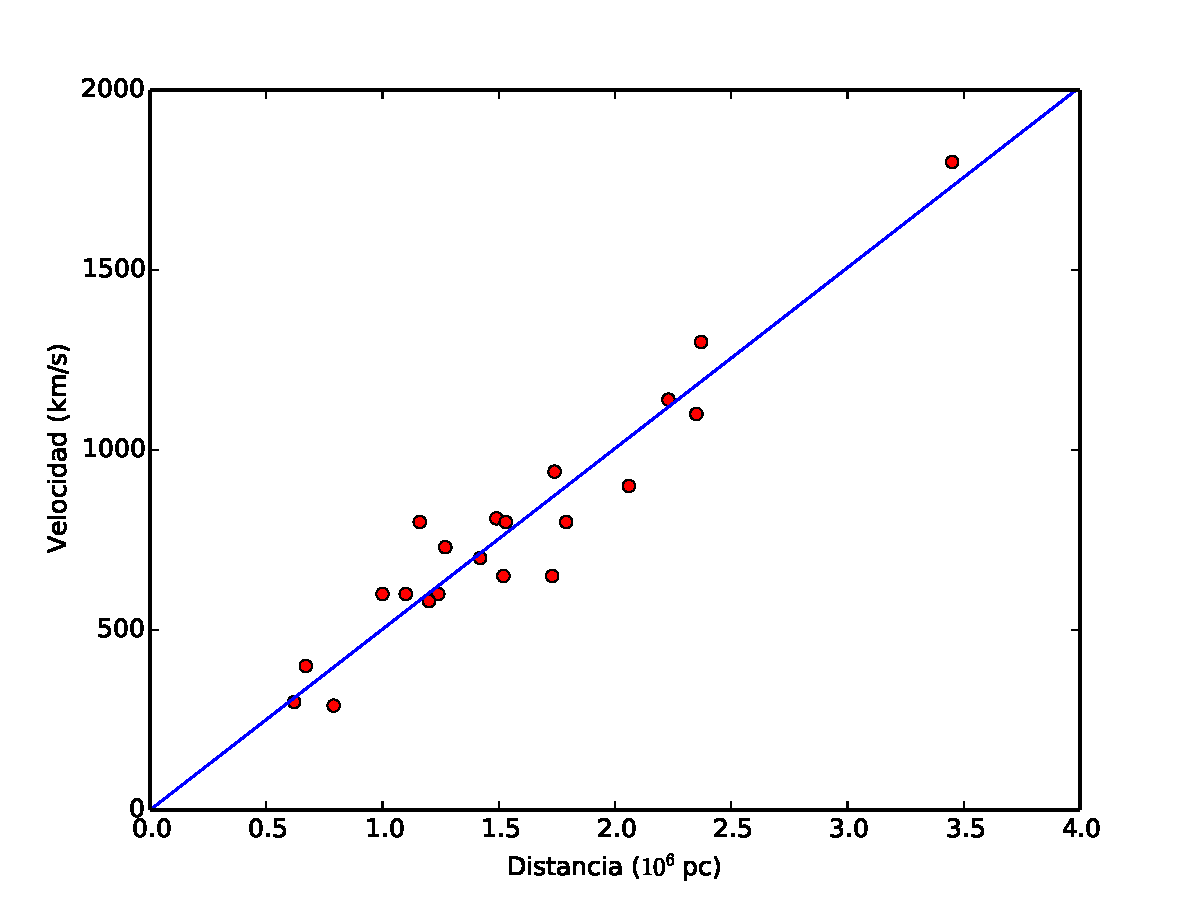
\includegraphics[width=0.7\textwidth]{fig/ajuste.pdf}
 \caption{Relaci'on entre la $velocidad$ y distancia de las nebulosas, medida por Hubble \cite{Hubble1}.}
  \label{hubble}
\end{figure}
Por otro lado, por comodidad es 'util definir el par'ametro adimensional $h$ tal que
\begin{equation}
H_0= 100 h \mbox{ km s}^{-1}\mbox{Mpc}^{-1} \label{h}
\end{equation}

%La figura (\ref{hubble}) muestra la recta originalmente ajustada por Hubble en 1929.
\section{Definiciones de Distancia}
Desde la aparici'on de la teor'ia de Relatividad Especial el concepto de distancia deja de ser una cantidad absoluta, por lo mismo 
se debe tener cuidado al momento de definir las distintas medidas de distancia usadas. En Cosmolog'ia la definici'on de distancia no es 'unica y se pueden 
emplear varios m'etodos para medirlas. Sus valores coinciden con la noci'on habitual de distancia para 
puntos cercanos ($r\ll 1$), pero difieren para puntos muy lejanos.\\
\subsection{Paralaje Trigonom'etrico}
El movimiento de la Tierra alrededor del Sol produce un movimiento aparente de la posici'on de alguna estrella alrededor
de una elipse. Para efectos pr'acticos se asume que la Tierra gira en una 'orbita circular cuyo radio es la distancia promedio
al Sol.
\begin{figure}[h]
  \centering
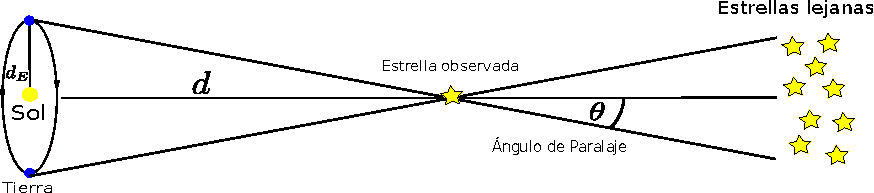
\includegraphics[width=0.8\textwidth]{fig/paralaje3.pdf}
 \caption{El movimiento de la Tierra alrededor del Sol.}
  \label{Paralaje}
  \end{figure}
Afortunadamente siempre la distancia de la Tierra a una estrella es mucho mayor que la distancia 
promedio de la Tierra al Sol (definida como \textit{Unidad Astron'omica}\footnote{$1\,AU= 1.496\times 10^{8}\,km$.} y simbolizada como $AU$) en ese caso el 'angulo de paralaje se puede aproximar
por la tangente entre ambos,
\begin{equation}
 \theta=\frac{d_{E}}{d},
\end{equation}
con $d_{E}$ la distancia Tierra-Sol y $d$ la distancia Tierra-Estrella.\\
A partir de esto podemos definir una nueva unidad de distancia, el \textit{P'arsec}\footnote{$1\,pc=206,264.8\,AU= 3.0856\times 10^{13}\,km = 3.2616\,\mbox{a\~nos luz}$.} (denotado con la sigla $pc$), como la distancia a la que 
debe estar un objeto para que el 'angulo de paralaje sea de $1"$. 
\subsection{Movimiento Propio}
Una fuente de luz a una distancia $d$ con  velocidad $v_{\bot}$ perpendicular a la l'inea de visi'on\footnote{L'inea recta imaginaria que une al observador con la estrella.}
parecer'a moverse a trav'es del cielo a una raz'on $\mu$ (en radianes/tiempo) dada por
\begin{equation}
\mu=\frac{v_{\bot}}{d}.
\end{equation}
Esto es conocido como movimiento propio. En general no se mide directamente esta cantidad, sino que la componente radial de la velocidad
$v_{\mbox{r}}$ a trav'es del efecto Doppler que genera el desplazamiento.\\ \\
'Ultimamente casi todas las mediciones de objetos dentro de nuestra galaxia se han efectuado usando alguno de estos dos m'etodos cl'asicos. Pero
si se desean medir la distancia a objetos mucho m'as lejanos dejan de ser adecuados, pues se basan en una visi'on cl'asica de un universo euclidiano.
\subsection{Luminosidad Aparente}
'Este es el m'etodo m'as usado para determinar distancias en Cosmolog'ia. Se basa en medir la potencia de luz emitida por un objeto,
cuya \textit{luminosidad absoluta} es conocida. La luminosidad absoluta $L$ se define como la potencia total radiada por el objeto 
(en todas direcciones). Entonces, asumiendo que la potencia radiada es la misma en todas direcciones podemos encontrar una simple 
relaci'on entre la potencia radiada total y la que recibir'ia un observador a una distancia $d$ del objeto.
\begin{equation}
l=\frac{L}{4\pi d^2}, \label{aparente}
\end{equation}
donde $l$ es la \textit{luminosidad aparente} recibida por el observador. Cabe se\~nalar que hemos considarado en esta 
expresi'on que el espacio es euclideano.
La expresi'on (\ref{aparente}) puede ser mejorada tomando en cuenta los efectos de la expansi'on del universo en la definici'on 
de $d$.\\ \\
Otro efecto importante a considerar es que un observador en la Tierra percibir'a una luminosidad aparente menor a la 
esperada por causa de la atm'osfera terrestre que absorbe parte de la luz recibida.
Se define la \textit{Magnitud Bolom'etrica} como la  magnitud aparente que tendr'ia una estrella si la radiaci'on
emitida por ella pudiera medirse en ausencia de la atm'osfera. Se representa por $M$ la magnitud absoluta y $m$ la aparente.\\
El astr'onomo brit'anico Norman Pogson en 1856 defini'o la escala moderna de magnitudes con base en la comparaci'on 
de luminosidades entre estrellas, de la cual se encuentra la relaci'on $l \propto 10^{2m/5}$. La constante 
de proporcionalidad pudo ser fijada en la d'ecada de 1930 con la llegada de las fotoceldas \cite{Hubble2}. 
De esta manera se obtuvo
\begin{equation}
l=10^{-2m/5}\times 2.52 \times 10^{-5} \left [\frac{erg}{cm^{2}s}\right ],
\end{equation}
 y la \textit{Magnitud bolom'etrica absoluta} $M$ 
\begin{equation}
L=10^{-2M/5}\times 3.02 \times 10^{35} \left [ \frac{erg}{s}\right ].
\end{equation}
Ambas expresiones son v'alidas para cualquier longitud de onda. Usando estas dos expresiones podemos reescribir (\ref{aparente}) como:
\begin{equation}
d=10^{1+(m-M)/5}pc.    \label{d}
\end{equation}
Hay muchos tipos de estrellas que son usadas para medir distancias a trav'es de la observaci'on de su luminosidad aparente.
\subsection{Velas Estandar}
'Estos son objetos estelares que pertenecen a una clase particular cuya luminosidad absoluta es conocida. Luego, por comparaci'on de luminosidades pueden ser
calculadas las distancias a otros objetos de la misma clase que se encuentren m'as lejanos a nuestra galaxia.
\paragraph{Cefeidas Variables:} Si se monitorea el brillo de ciertas estrellas, veremos que 'este oscila en el tiempo.
'Estas son conocidas como \textit{Estrellas variables}. El periodo de luminosidad puede variar desde minutos a meses o incluso
a\~nos. Dentro de este tipo de estrellas se encuentran las Cefeidas variables, cuyos periodos de luminosidad var'ian entre 1
a 100 d'ias y en nuestra galaxia se han encontrado  m'as de 1000.\\
Cuando se estudian las l'ineas espectrales en Cefeidas, se detectan corrimientos que var'ian con el mismo periodo que el de su 
luminosidad. Esto nos indica que la superficie de esta estrella se mueve, es decir, la luminosidad cambia como cambia la superficie
de la estrella.\\
Para entender esto consideremos una estrella com'un y corriente de radio $R_{0}$ y supongamos que 'esta es perturbada cambiando
su radio a $R$, tal que $R<R_{0}$, entonces debido a esta perturbaci'on su densidad y presi'on aumentar'an. El exceso en la presi'on
har'a que se expanda sobrepasando el radio de $equilibrio$ $R_{0}$. La disminuci'on en la presi'on generar'a que se vuelva
a comprimir, repiti'endose este proceso sucesivas veces.\\
En el an'alisis anterior dejamos de lado efectos importantes como la Opacidad\footnote{Un material presenta opacidad cuando no deja pasar luz en proporci'on apreciable.}.
En estrellas normales, la opacidad disminuye al aumentar la temperatura, esto significa, al comprimirse la estrella a causa del
aumento de presi'on tambi'en aumentar'a la temperatura y por lo tanto disminuir'a la opacidad. De este modo, cuando la estrella se expande
disminuye la presi'on y la temperatura, provocando un aumento en la opacidad. Esto genera los cambios peri'odicos en su luminosidad \cite{ceph2}.\\
En particular, las Cefeidas son un tipo de estrella variable con una gran luminosidad y por lo mismo son unas de las  m'as
usadas para medir distancias fuera de nuestra galaxia.
Adem'as, su periodo de luminosidad tiene una estrecha relaci'on con la misma luminosidad: entre mayor sea el periodo, mayor ser'a su luminosidad.
Calibrando la relaci'on entre luminosidad-periodo de Cefeidas cercanas se puede calcular la luminosidad de otras m'as lejanas
a trav'es de su periodo y por lo tanto nos permiten establecer distancias a trav'es de su luminosidad.
\begin{figure}[h!]
  \centering
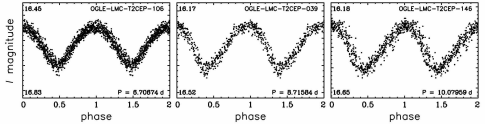
\includegraphics[width=0.8\textwidth]{fig/cepheid.png}
 \caption{Curvas de luz de tres Cefeidas ordinarias tipo II, con periodos similares \cite{ceph}.}
  %\label{}
  \end{figure}\\
\paragraph{Supernova Ia:} Se cree que ocurre cuando una enana blanca en un sistema binario aumenta su masa absorbiendo la de su
compa\~nera hasta acercarse al l'imite de Chandrasekhar\footnote{Es la m'axima masa posible de una estrella fr'ia estable. Si la estrella supera este l'imite  colapsa.}.
Cuando esto ocurre la enana blanca se vuelve inestable, aumentando su temperatura y densidad, generando explosiones
termonucleares las cuales pueden abarcar distancias de varios megaparsecs. Como todas estas estrellas explotan en condiciones
similares, la luminosidad de sus explosiones variar'an muy poco unas de otras, haciendo de las supernovas Ia un buen indicador de distancias.
\subsection{Distancia de Luminosidad}
Cuando se miden distancias con redshifts considerables ($z>0.1$) lo efectos de la expansi'on cosmol'ogica no pueden ser 
despreciados. Anteriormente encontramos una relaci'on entre la luminosidad absoluta y la luminosidad aparente (\ref{aparente})
a una distancia $d$, a la cual debemos hacer algunas correcciones.\\ \\
Imaginemos una estrella con coordenadas $\vec{x}_{1}=(ct_{1},r_{1},0,0)$ (en coordenadas esf'ericas), y que la tierra
se encuentra en las coordenadas $\vec{x}_{0}=(ct_{0},0,0,0)$, considerando (\ref{dsFRW}), la m'etrica inducida por una esfera centrada
(para un tiempo fijo) en $\vec{x}_{1}$ y que pasa por $\vec{x}_{0}$ ser'a 
\begin{equation}
 dl^2=a_{0}^2 r_{1}^2(d\theta^2  +\sen^2\theta d\varphi^2),\hspace{0.5cm} \mbox{con} \hspace{0.5cm}  a_{0}= a(t_{0}),
\end{equation}
cuya 'area es
\begin{equation}
A=4\pi a_{0}^2 r_{1}^2 . 
\end{equation}
Por otro lado, si la estrella emite $N$ fotones, de fecuencia $\nu_{1}$, en un intervalo de tiempo $\delta t_{1}$, la 
luminosidad absoluta ser'a:
\begin{equation} 
L=\frac{N h\nu_{1}}{\delta t_{1}}  \hspace{0.2cm} \Rightarrow \hspace{0.2cm} N=\frac{L\delta t_{1}}{h\nu_{1}},\label{Ltotal}
\end{equation}
con $h$ la constante de Planck. Un observador en $\vec{x}_{0}$ detectar'a $n$ fotones ($n<N$) en un 'area $S$ con frecuencia $\nu_{0}$, a causa del redshift,
en un intervalo de tiempo $\delta t_{0}$. Adem'as, al ser el espacio is'otropo cualquier observador que se encuentre en la superficie
esf'erica que encierra a la estrella recibir'a los mismos $n$ fotones con la misma frecuencia en el mismo intervalo de tiempo y superficie. As'i,
asumiendo que no hay p'erdida de fotones, por esta superficie esf'erica deber'an pasar en total $N$ fotones en el intervalo
de tiempo $\delta t_{0}$, es decir,
\begin{equation}
\int_{A}\frac{n}{S}dA=4\pi a_{0}^2 r_{1}^2 \frac{n}{S}= N.
\end{equation}
Entonces, podemos escribir la luminosidad aparente como
\begin{equation}
 l=\frac{nh\nu_{0}}{S\delta t_{0}} =\frac{Nh\nu_{0}}{4\pi a_{0}^2r_{1}^2\delta t_{0}}  \hspace{0.2cm} \Rightarrow \hspace{0.2cm} N=\frac{4\pi l a_{0}^2r_{1}^2\delta t_{0}}{h\nu_{0}},\label{laparente} 
\end{equation}
igualando (\ref{Ltotal}) y (\ref{laparente}) obtenemos
\begin{equation}
l=\frac{L}{4\pi a_{0}^2 r_{1}^2}\frac{\delta t_{1}}{\delta t_{0}}\frac{\nu_{0}}{\nu_{1}}.
\end{equation}
Adem'as, podemos relacionar $\delta t_{1}/\delta t_{0}$ y $\nu_{0}/\nu_{1}$ con el redshift cosmol'ogico usando (\ref{zc}) y (\ref{62i})
respectivamente. Con esto, encontramos la relaci'on
\begin{equation}
l =\frac{L}{4\pi a_{0}^2 r_{1}^2 (1+z)^2}.
\end{equation}
En base a este resultado, podemos definir la \textit{distancia de luminosidad} como
\begin{equation}
d_{L} :=  a_{0} r_{1} (1+z), \label{dl}
\end{equation}
tal que 
\begin{equation}
l=\frac{L}{4\pi d_{L}^2}.
\end{equation}
Por otro lado, usando (\ref{dl}) y (\ref{d}) podemos expresar la distancia de luminosidad en funci'on de las magnitudes absolutas y relativas de las estrellas.
\begin{equation}
m-M = 5\log\left(\frac{d_L(z)}{1pc}\right) - 5. \label{m-M}
\end{equation}
Esta definici'on de distancia resulta muy 'util para encontrar una relaci'on entre distancia y redshifts. Ahora la utilizaremos
en el caso particular en que $z\ll1$, para expandir en serie de potencias a segundo orden en $(t-t_{0})$:\\
\begin{eqnarray}
 a(t)&=&a(t_0)+\dot{a}(t_0)(t-t_0)+\frac{1}{2}\ddot{a}(t_0)(t-t_0)^2+\cdots \\
&=& a(t_0)\left[1+H_0(t-t_0)-\frac{1}{2}q_0H_0^2(t-t_0)^2+\cdots\right]. 
\end{eqnarray}
Aqu'i hemos definido el \textit{par'ametro de desaceleraci'on} $q_0$ como 
\begin{equation}
q_0:=-\frac{a(t_0)}{\dot{a}^2(t_0)}\ddot{a}(t_0).\label{q0}
\end{equation}
Luego,
\begin{equation}
\frac{a(t)}{a(t_0)}=1+H_0(t-t_0)-\frac{1}{2}q_0H_0^2(t-t_0)^2+\cdots .\label{z2}
\end{equation}
Pero $1+z=a(t_0)/a(t)$. Entonces, invirtiendo (\ref{z2}) encontramos
\begin{eqnarray}
 \frac{a(t_0)}{a(t)}&=&\left[1+H_0(t-t_0)-\frac{1}{2}q_0H_0^2(t-t_0)^2+\cdots\right]^{-1} \\
&=& 1+H_0(t_0-t)+\frac{1}{2}(q_0 +2)H_0^2(t_0-t)^2+ O\left[(t-t_{0})^3\right]\\
\Rightarrow z&\approx&H_0(t_0-t)+\frac{1}{2}(q_0 +2)H_0^2(t_0-t)^2.   \label{z3}
\end{eqnarray}
Esta expresi'on puede ser invertida\footnote{Basta con encontrar las raices de esta expresi'on y expandir a segundo orden en potencias de $z$.} expresando $t$ en funci'on de $z$
\begin{equation}
 H_{0}(t_0 -t)\approx  z -\frac{1}{2}(q_0 +2)z^2.
\end{equation}
Pero lo que deseamos hacer es relacionar la distancia de luminosidad con el redshift, para ello usaremos (\ref{60i}), que adopta la forma
\begin{equation}
\frac{c}{a(t_0)}\int_{t_1}^{t_0}\left[H_{0}t+\frac{1}{2}H_{0}^{2}(q_0 +2)t^2\right]dt \approx r_1.
\end{equation}
Como aproximamos a segundo orden en $(t-t_{0})$, podemos escribir
\begin{equation}
  \frac{r_1}{c} \approx \frac{t_0 -t_1}{a(t_0)} +\frac{H_{0}(t_0 -t_1)^2}{2a(t_0)}.\\
\end{equation}
\begin{equation}
   \frac{r_1}{c} a(t_0) H_0 \approx z -\frac{1}{2}(1+ q_0)z^2. \hspace{0.5cm}
\end{equation}
Manteniendo la aproximaci'on a segundo orden en $z$ y usando la definici'on de distancia de luminosidad (\ref{dl}) encontramos
\begin{equation}
d_{L}\approx \frac{c}{H_0}\left[z+\frac{1}{2}(1-q_0)z^2 \right]. \label{dlq0}
\end{equation}
Esta expresi'on tiene una buena precisi'on hasta redshifts de 0.2, para mayores valores la expansi'on en serie de potencias no es 'util.

\subsection{Distancia Angular}
Otra noci'on simple de distancia es la \textit{distancia angular}. Ella requiere conocer el tama\~no (lineal) ``real'' $D$
de un objeto (por ejemplo, una galaxia), entendido como su tama\~no medido por un observador que se mueve con el objeto. 
Si respecto a un observador lejano el objeto subtiende un 'angulo $\Delta\varphi$ entonces definimos la distancia angular
desde el observador al objeto como $d_A:=D/\Delta\varphi$.
\begin{figure}[h]
  \centering
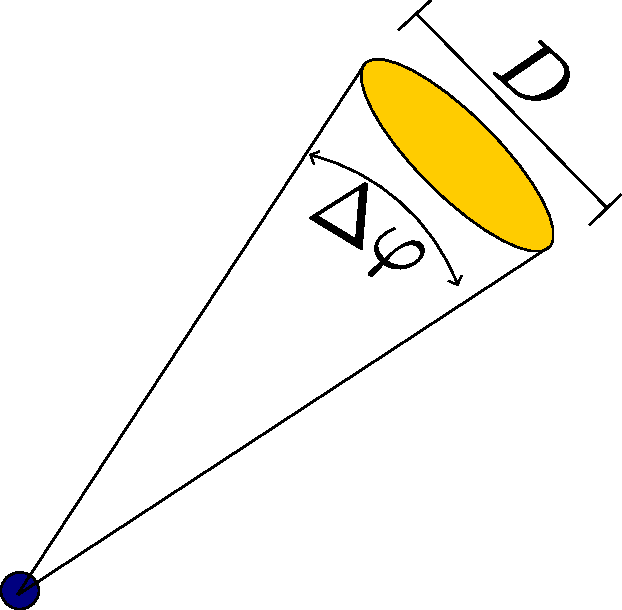
\includegraphics[width=0.3\textwidth]{fig/dangular.pdf}
 \caption{El punto azul representa la tierra mientras que el amarillo el objeto en estudio.}
 % \label{}
  \end{figure}\\
  Un c'alculo simple muestra que un objeto ubicado en la coordenada
$r_1$ en el tiempo $t_1$ tendr'a distancia angular dada por
\begin{equation}\marginnote{distancia angular}
 d_A=a(t_1)r_1.
\end{equation}

Es claro que tanto $d_L$ como $d_A$ coinciden con la definici'on usual de distancia si estamos en un 
universo plano sin expansi'on. Tambi'en es importante notar que para determinar tanto $d_A$ como $d_L$ es necesario 
conocer \textit{propiedades int'insecas} del objeto. Para calcular la distancia angular se requiere conocer el tama\~no
``real'' $D$ del objeto, mientras que para determinar la distancia de luminosidad se requiere la luminosidad absoluta $L$.

%\subsection{Relaci'on distancia de luminosidad - redshift}

%\begin{eqnarray}
% a(t)&=&a(t_0)+\dot{a}(t_0)(t-t_0)+\frac{1}{2}\ddot{a}(t_0)(t-t_0)^2+\cdots \\
%&=& a(t_0)\left[1+H_0(t-t_0)-\frac{1}{2}q_0H_0^2(t-t_0)^2+\cdots\right], \label{expR}
%\end{eqnarray}
%donde hemos definido la \textit{constante de Hubble} y el \textit{par'ametro de desaceleraci'on} por
%\begin{equation}
% H_0:=\frac{\dot{a}(t_0)}{a(t_0)},
%\end{equation}
%\begin{equation}
%q_0:=-\frac{a(t_0)}{\dot{a}^2(t_0)}\ddot{a}(t_0).
%\end{equation}
%Usando (\ref{expR}) podemos reescribir (\ref{zc}) como
%\begin{equation}
% z=H_0(t_0-t_1)+\left(1+\frac{q_0}{2}\right)H_0^2(t_0-t_1)^2+\cdots
%\end{equation}
%Invirtiendo esta expresi'on, encontramos
%\begin{equation}
% t_0-t_1=\frac{1}{H_0}\left[z-\left(1+\frac{q_0}{2}\right)z^2+\cdots\right].
%\end{equation}
%Con esto, podemos expresar la integral como
%\begin{equation}
% f(r_1)=\frac{c}{a(t_0)}\left[(t_0-t_1)+\frac{1}{2}H_0(t_0-t_1)^2+\cdots\right]
%\end{equation}
%\begin{equation}
% f(r_1)=\frac{c}{a(t_0)H_0}\left[z-\frac{1}{2}(1+q_0)z^2+\cdots\right]
%\end{equation}
%\begin{equation}
%d_L=\frac{c}{H_0}\left[z+\frac{1}{2}(1-q_0)z^2+\cdots\right]
%\end{equation}

\section{Ecuaciones de Einstein}

Como bien dijimos al principio del cap'itulo, a escalas cosmol'ogicas el universo (visto por observadores com'oviles con el fluido cosmol'ogico) luce homog'eneo e is'otropo. 
Esto implica que el tensor de energ'ia-mom'entum del fluido cosmol'ogico debe poseer estas mismas propiedades. Si suponemos que
el fluido cosmol'ogico es un fluido perfecto con presi'on $p$ y densidad de masa $\rho$, las componentes de su tensor energ'ia-mom'entum, debido a que la m'etrica
de espaciotiempo  es diagonal, ver (\ref{dsFRW}), ser'an
\begin{eqnarray}
T^{00}=\rho(t)c^2,\qquad T^{0i}=0, \qquad T^{ij}= -g^{ij}p(t),
\end{eqnarray}
donde $p$ y $\rho$ s'olo pueden depender del tiempo (por la isotrop'ia y homogeneidad). $T^{0i}=0$ tambi'en nos indica que el fluido cosmol'ogico
est'a en reposo respecto a observadores com'oviles con 'el ($u^\mu=(u^0,0,0,0)$).
De este modelo del universo podemos extraer informaci'on interesante. De la ec. de balance de la energ'ia %por ejemplo usando (\ref{dcT0})
\begin{eqnarray}
0 = \nabla_\mu T^{0\mu}&=& \frac{\partial T^{0\mu}}{\partial x^\mu} + \Gamma^{0}_{\mu\nu} T^{\nu \mu} + \Gamma^{\mu}_{\mu \nu} T^{0\nu}\\
                   &=& \frac{\partial T^{00}}{\partial x^0} + \Gamma^{0}_{ij} T^{ij} + \Gamma^{i}_{i0} T^{00},\\
\end{eqnarray}
obteniendo finalmente\footnote{Cabe mencionar que usando (\ref{a1}) y (\ref{a2}) tambi'en se puede obtener (\ref{rho}).}
\begin{equation}
\boxed{\dot \rho +3\frac{\dot a}{ac^2}(p+\rho c^2)= 0.} \label{rho} 
\end{equation}
Asumiendo la ecuaci'on de estado politr'opica
\begin{equation}
p=c^2\omega \rho,
\end{equation}
siendo $\omega$ independiente del tiempo, podemos encontrar una relaci'on entre $\rho$ y $a$ a partir de (\ref{rho}):
\begin{equation}
\rho =\rho_0 \left(\frac{a}{a_0}\right)^{-3(1+\omega)}.
\end{equation}
En el caso en que el fluido cosmol'ogico est'a compuesto mayoritariamente por materia no-relativista ($p\ll \rho c^{2}$), entonces $\omega \ll 1$ y por lo tanto
\begin{equation}
\rho =\rho_0 \left(\frac{a}{a_0}\right)^{-3}, \label{materia}
\end{equation}
o bien si fuese predominante la materia relativista ($p=c^{2}\rho/3$ , es decir $\omega = 1/3$)
\begin{equation}
\rho =\rho_0 \left(\frac{a}{a_0}\right)^{-4}. \label{radiacion}
\end{equation}
Por otro lado, de las ecuaciones de Einstein se puede obtener m'as informaci'on sobre la din'amica de la expansi'on del universo. De la componente $\mu=\nu=0$ de (\ref{EE3})
 y usando las conexiones calculadas anteriormente,
\begin{equation}
R_{00}=\frac{\partial\Gamma_{00}^\lambda}{\partial x^\lambda} -\frac{\partial\Gamma_{0\lambda}^\lambda}{\partial x^0}  +\Gamma^\lambda_{\lambda\rho}\Gamma^\rho_{00}  -\Gamma^\lambda_{0\rho}\Gamma^\rho_{0\lambda},          
\end{equation}
se obtiene
\begin{equation}
R_{00}=-\frac{3}{c^2}\frac{\ddot a}{a}.
\end{equation}
Adem'as,
\begin{equation}
T_{00}-\frac{1}{2}g_{00}T=\frac{4\pi G}{c^4}(\rho c^2+3p).
\end{equation}
Por lo tanto,
\begin{equation}
\boxed{\frac{3\ddot a}{a}=-\frac{4\pi G}{c^2}(\rho c^2+3p).} \label{a1}
\end{equation}
Por otro lado, sabemos que $T_{0i}=0$ y por los mismos motivos de homogeneidad del espacio $R_{0i}$ debe ser $0$. As'i, s'olo 
falta calcular $R_{ij}$,
\begin{equation}
R_{ij}=\frac{\partial\Gamma_{ij}^\lambda}{\partial x^\lambda} -\frac{\partial\Gamma_{j\lambda}^\lambda}{\partial x^i}  +\Gamma^\lambda_{\lambda\rho}\Gamma^\rho_{ij}  -\Gamma^\lambda_{i\rho}\Gamma^\rho_{j\lambda},   
\end{equation}
\begin{equation}
R_{ij}= \left[2k +\frac{2}{c^2}\dot a^2 +\frac{1}{c^2}a\ddot a\right] \mbox{\~g}_{ij},
\end{equation}
con $\mbox{\~g}_{ij}=\mbox{g}_{ij}/a^2$, adem'as
\begin{equation}
T_{ij}-\frac{1}{2}g_{ij}T=\frac{a^2}{2c^2}(\rho c^2- p)\mbox{\~g}_{ij}.
\end{equation}
Por lo tanto,
\begin{equation}
\boxed{\frac{2kc^2}{a^2} +\frac{2\dot a^2}{a^2} +\frac{\ddot a}{a}= \frac{4\pi G}{c^2}(\rho c^2- p).} \label{a2}
\end{equation}
Usando (\ref{a1}) y (\ref{a2}) se pueden eliminar las segundas derivadas, obteniendo
\begin{equation}
\boxed{\dot a^2 +kc^2  = \frac{8\pi G\rho a^2}{3}.} \label{dota}
\end{equation}
'Esta es la ecuaci'on fundamental de Friedmann \cite{friedmann} que gobierna la expansi'on del universo.\\
De aqu'i vemos que la expansi'on s'olo puede detenerse en un universo con curvatura positiva, es decir $k=1$.\\
En base a (\ref{dota}) podemos definir la \textit{densidad de masa cr'itica} actual como
\begin{equation}
\rho_{0\rm{,crit}}:= \frac{3H_0^2}{8\pi G} = 1.878\times 10^{-29} h^2 \mbox{ g/cm}^3,
\end{equation}
donde $h$ es la constante de Hubble en unidades de $100$ km s$^{-1}$Mpc$^{-1}$. Es llamada as'i pues despejando $\rho$ de
(\ref{dota}) se obtiene
\begin{equation}
\rho = \frac{3\dot a^2}{8\pi Ga^2} + \frac{3kc^2}{8\pi Ga^2}, \label{densidad}
\end{equation}
lo que significa que
\begin{equation}
\rho_0 = \frac{3 H_0^2}{8\pi G} + \frac{3kc^2}{8\pi Ga_0^2} = \rho_{0\rm{,crit}} + \frac{3kc^2}{8\pi Ga_0^2}. 
\end{equation}
Si $\rho_0 > \rho_{0\rm{,crit}}$ estamos en un universo con curvatura espacial positiva.
Si $\rho_0=\rho_{0\rm{,crit}}$ estamos en un universo espacialmente plano. Si $\rho_0<\rho_{0\rm{,crit}}$ estamos en un universo curvatura espacial negativa.
Es decir, $\rho_{0\rm{,crit}}$ es un \textit{punto de inflecci'on} para el valor de la densidad, entre estos tres posibles casos.\\
De la definici'on (\ref{q0}) y la ec. (\ref{a1}) encontramos la expresi'on
\begin{equation}
q_{0}=\frac{4\pi G}{3c^2 H_0^2}(\rho_0 c^2 +3p_0)=\frac{\rho_0 c^2 +3p_0}{2\rho_{0\rm{,crit}}} . \label{q00}
\end{equation}

Por otro lado, analizando (\ref{a1}) vemos que este modelo s'olo permite una expansi'on desacelerada, ya que, si $c^2\rho+ 3p$ proviene de una mezcla de
radiaci'on y materia $q_0>0$ y $\ddot a<0$. Esto tiene mucho sentido, pues en ausencia de cualquier otro tipo de fuerzas, la
atracci'on gravitacional ser'a la 'unica que domine el comportamiento del universo a escalas cosmol'ogicas.\\
Otra de las consecuencias de este modelo es que la edad actual del 
universo es mayor que el tiempo de Hubble. Si graficamos  $a(t)/a_0$ vs $t$ entonces $H_0$ es la pendiente de la curva en $t_0$,
por lo tanto cualquier modelo del universo debe tener dicha pendiente en $t_0$.\\
\begin{figure}[h!]
  \centering
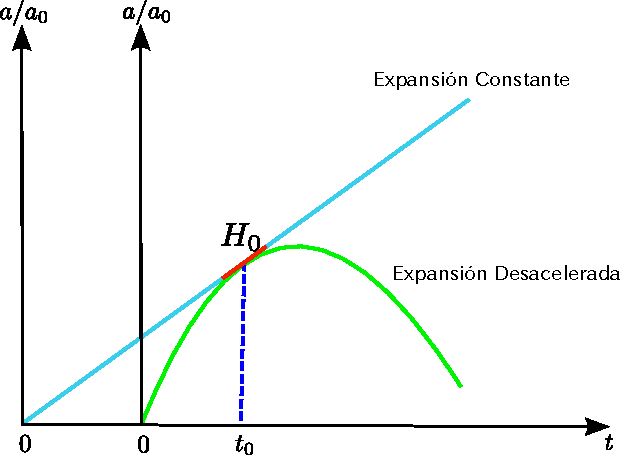
\includegraphics[width=0.55\textwidth]{fig/ex.pdf}
 \caption{Como se puede observar del gr'afico, si la expansi'on es desacelerada el tiempo transcurrido desde $a=0$ hasta $a_0$ es menor que el de un modelo de expansi'on a velocidad constante.}
 % \label{}
  \end{figure}\\
Como ya hemos visto, actualmente se sabe que la expansi'on del universo no es desacelerada,
por el contrario, el universo se expande en forma acelerada, por lo que el modelo propuesto no se ajusta a las observaciones.
Esto puede ser solucionado agregando la Constante Cosmol'ogica $\Lambda$ a las ecuaciones de Einstein\footnote{Ver ecuaci'on (\ref{EE2}).}
tal que $\ddot a > 0$. Esta constante tiene dos interpretaciones distintas. 
La primera, es que 'esta es una correcci'on a las ecuaciones de Einstein, la que s'olo es significativa a escalas cosmol'ogicas. 
La segunda, requiere poner esta constante al otro lado de la igualdad,
\begin{equation}
R_{\mu \nu} -\frac{1}{2}Rg_{\mu \nu} = \frac{8\pi G}{c^4}T_{\mu \nu}+ \Lambda g_{\mu \nu} = \frac{8\pi G}{c^4}T^{\prime}_{\mu \nu}, \label{TEL}
\end{equation}
as'i $T^{\prime}_{\mu \nu}$ corresponde al tensor energ'ia-mom'entum de la materia que conforma el universo conocido m'as 
otro tipo de \textquotedblleft materia\textquotedblright  con densidad de masa y presi'on tales que $\ddot a > 0$.\\
En ese caso, el tensor de energ'ia-mom'entum de este fluido desconocido ser'ia
\begin{equation}
T^{\Lambda}_{\mu\nu}=\frac{c^4\Lambda}{8\pi G} g_{\mu\nu}.
\end{equation}
Puede identificarse este energ'ia-mom'entum como el de un fluido perfecto con densidad y presi'on dadas por,
\begin{eqnarray}
\rho_{\Lambda}=\frac{c^2\Lambda}{8\pi G},    \qquad
p_{\Lambda}=-\frac{c^4\Lambda}{8\pi G}.
\end{eqnarray}
Por lo que este supuesto fluido satisface una ec. de estado politr'opica,
\begin{equation}
p=-\rho c^2,
\end{equation}
es decir, aqu'i  $\omega=-1$.\\
Entonces, si aparte del fluido cosmol'ogico agregamos este nuevo fluido a (\ref{a1}), obtenemos
\begin{equation}
\frac{3\ddot a}{a}=-\frac{4\pi G}{c^2}(\rho c^2+3p)+\Lambda c^2. 
\end{equation}
Entonces, para que $\ddot a$ sea mayor a cero $\Lambda$ debe satisfacer
\begin{equation}
\Lambda > \frac{4\pi G}{c^4}(\rho c^2 + 3p),
\end{equation}
Esto significa que $\Lambda$ debe ser una constante positiva, y por consiguiente genera presi'on efectiva negativa, tal que
contrarresta la atracci'on gravitacional.\\ \\
Ahora bien, supongamos que el universo est'a conformado por materia relativista y materia no-relativista las cuales no interactuan en forma significativa entre ellas  y adem'as agregamos la constante cosmol'ogica, entonces

\begin{equation}
\rho = \rho_{\rm{R}} + \rho_{\rm{M}} + \rho_{\rm{\Lambda}},
\end{equation}
aqu'i $\rho_{\rm{R}}$ representa la densidad de masa de la materia relativista, $\rho_{\rm{M}}$ la densidad de masa de la materia no relativista y $\rho_\Lambda$ representa una densidad de masa efectiva a causa de la constante cosmol'ogica. Reemplazando con (\ref{materia}) y (\ref{radiacion}), encontramos
\begin{equation}
\rho = \rho_{0\,\rm{R}}\left(\frac{a_0}{a}\right)^{4} + \rho_{0\,\rm{M}}\left(\frac{a_0}{a}\right)^{3} + \rho_{\rm{\Lambda}}.
\end{equation}
Podemos reescribir la densidad de masa como:
\begin{equation}
\rho = \frac{3H_0^2}{8\pi G}\left[\Omega_{\rm{R}}\left(\frac{a_0}{a}\right)^{4} + \Omega_{\rm{M}}\left(\frac{a_0}{a}\right)^{3} + \Omega_{\rm{\Lambda}}\right], \label{ro0}
\end{equation}
con
\begin{eqnarray}
\Omega_{\rm{R}} := \frac{3H_0^2\rho_{0\,\rm{R}}}{8\pi G},\qquad 
\Omega_{\rm{M}} := \frac{3H_0^2\rho_{0\,\rm{M}}}{8\pi G}, \qquad
\Omega_{\rm{\Lambda}} := \frac{3H_0^2 \rho_{0\,\rm{\Lambda}}}{8\pi G},
\end{eqnarray}
tal que al evaluar (\ref{dota}) en $t_0$ obtenemos
\begin{equation}
\hspace{2cm} \Omega_{\rm{R}} +\Omega_{\rm{M}} +\Omega_{\rm{\Lambda}} +\Omega_{\rm{k}} =1, \hspace{1cm} \mbox{con} \hspace{0.2cm} \Omega_{\rm{k}} := -\frac{kc^2}{a_0^2H_0^2}. 
\end{equation}
Adem'as, podemos escribir la presi'on actual como
\begin{equation}
p_0=\frac{3H_0^2}{8\pi G}\left( -\Omega_{\rm{\Lambda}}  +\frac{1}{3}\Omega_{\rm{R}} \right). \label{p0}
\end{equation}
Reemplazando (\ref{p0}) y (\ref{ro0}) en (\ref{q00}), se obtiene que
\begin{equation}
q_0=\frac{1}{2}(\Omega_{\rm{M}} + 2\Omega_{\rm{R}}  - 2\Omega_{\rm{\Lambda}}).  \label{q0omega}
\end{equation}
Por otro lado, usando (\ref{dota}) vemos que
\begin{equation}
 \dot a^2 = H_0^2 a^2\left[\Omega_{\rm{R}}\left(\frac{a_0}{a}\right)^{4} + \Omega_{\rm{M}}\left(\frac{a_0}{a}\right)^{3} + \Omega_{\rm{\Lambda}} +\Omega_{\rm{k}}\left(\frac{a_0}{a}\right)^{2} \right]. 
\end{equation}
Luego, definiendo $x=:a/a_0$, podemos escribir 
\begin{equation}
\dot x^2 =H_0^2 x \left[\Omega_{\rm{R}}x^{-4} + \Omega_{\rm{M}}x^{-3}  +\Omega_{\rm{k}}x^{-2} + \Omega_{\rm{\Lambda}}\right].
\end{equation}
Usando (\ref{zc}) y despejando $t$ en funci'on de $z$, obtenemos
\begin{equation}
t(z)=\frac{1}{H_0}\int_0^{1/(1+z)}\frac{dx}{x\sqrt{\Omega_{\rm{R}}x^{-4} + \Omega_{\rm{M}}x^{-3}+\Omega_{\rm{k}}x^{-2} + \Omega_{\rm{\Lambda}} }}.
\end{equation}
Esta expresi'on nos permite calcular la edad actual del universo como
\begin{equation}
t_0=\frac{1}{H_0}\int_0^1\frac{dx}{x\sqrt{\Omega_{\rm{R}}x^{-4} + \Omega_{\rm{M}}x^{-3}+\Omega_{\rm{k}}x^{-2} + \Omega_{\rm{\Lambda}} }}. \label{tiempo}
\end{equation}
Por otro lado, de (\ref{60i}) vemos que
\begin{equation}
f(r(z))=c\int_{t_0}^{t(z)}\frac{dt}{a(t)}= \frac{c}{a_0H_0}\int_{1/(1+z)}^1\frac{dx}{x^2\sqrt{\Omega_{\rm{R}}x^{-4} + \Omega_{\rm{M}}x^{-3}+\Omega_{\rm{k}}x^{-2} + \Omega_{\rm{\Lambda}} }}.
\end{equation}
Luego,
\begin{equation}
r(z)=S\left[\frac{c}{a_0H_0}\int_{1/(1+z)}^1\frac{dx}{x^2\sqrt{\Omega_{\rm{R}}x^{-4} + \Omega_{\rm{M}}x^{-3}+\Omega_{\rm{k}}x^{-2} + \Omega_{\rm{\Lambda}} }}\right],
\end{equation}
con
\begin{equation}
S\left[y\right]=\left\{
\begin{array}
[c]{ccl}%
\text{sen}(y), &\text{si}& k=+1\\
y, &\text{si}& k=0\\
\text{senh}(y), &\text{si}& k=-1
\end{array}
\right. . \label{61i2}%
\end{equation}
Entonces, usando la definici'on de distancia de luminosidad (\ref{dl}), encontramos
\begin{equation}
d_L(z)=a_0(1+z)S\left[\frac{c}{a_0H_0}\int_{1/(1+z)}^1\frac{dx}{x^2\sqrt{\Omega_{\rm{R}}x^{-4} + \Omega_{\rm{M}}x^{-3} +\Omega_{\rm{k}}x^{-2} + \Omega_{\rm{\Lambda}}}}\right]. \label{dlzk}
\end{equation}
En particular para el caso $k=0$ tenemos que $\Omega_k=0$ y por lo tanto
\begin{equation}
\boxed{d_L(z)=\frac{(1+z)c}{H_0}\int_{1/(1+z)}^1\frac{dx}{x^2\sqrt{\Omega_{\rm{R}}x^{-4} + \Omega_{\rm{M}}x^{-3} + \Omega_{\rm{\Lambda}}}}.} \label{dlz}
\end{equation}



%\begin{align}
%G_{00} &= \frac{3}{c^2}\left(\frac{\dot{a}^2}{a^2}+\frac{kc^2}{a^2}\right), \\
%G_{rr} &=-\frac{1}{c^2(1-kr^2)}\left(2R\ddot{a}+\dot{a}^2+kc^2\right) = \frac{g_{rr}}{c^2}\left(2a\ddot{a}+\dot{a}^2+kc^2\right), \\
%G_{\theta\theta} &= -\frac{r^2}{c^2}\left(2a\ddot{a}+\dot{a}^2+kc^2\right) 
%=\frac{g_{\theta\theta}}{c^2}\left(2a\ddot{a}+\dot{a}^2+kc^2\right) , \\
%G_{\varphi\varphi} &= G_{\theta\theta}\sen^2\theta
%=\frac{g_{\varphi\varphi}}{c^2}\left(2a\ddot{R}+\dot{a}^2+kc^2\right).
%\end{align}

%\begin{align}
%T_{00} &= \rho c^2, \\
%T_{rr} &= -p\, g_{rr}, \\
%T_{\theta\theta} &= -p\, g_{\theta\theta}, \\
%T_{\varphi\varphi} &= -p\, g_{\varphi\varphi}.
%\end{align}
\section{Datos experimentales, Modelos y Ajustes}
         
Como hemos visto, este modelo cosmol'ogico nos permite obtener mucha informaci'on sobre el universo, sobre su curvatura, su edad y tipo de 
materia que lo compone. Entonces es momento de poner a prueba nuestros modelos del universo, usando los datos experimentales.\\ \\
El Proyecto Cosmol'ogico de Supernovas (Supernova Cosmology Project\footnote{Sitio web: \url{http://supernova.lbl.gov/}.} o abreviado por sus siglas SCP) es uno de los dos equipos de investigaci'on que determinaron
que el universo se expande en forma acelerada. Ellos usaron cientos de datos tomados del redshift de supernovas tipo Ia.
El SCP Union2.1 SN Ia\footnote{Direcci'on web: \url{http://supernova.lbl.gov/Union/}.} es una compilaci'on de datos obtenidos de las supernovas Ia.
Como se puede ver en el link al pie de la p'agina, estos datos est'an en una tabla donde la primera columna corresponde al nombre de la
supernova, la segunda al redshift medido, la tercera columna corresponde a la cantidad $m-M$ y la cuarta columna corresponde al error asociado a la medici'on de $m-M$.
\begin{equation}
\begin{array}{lccl}
\mbox{Nombre} & z        &     m-M       & \mbox{Error } m-M\\
1993\mbox{ah} & 0.028488 & 35.3465833928 & 0.223905932998	\\
1993\mbox{ag} & 0.050043 & 36.6823679154 & 0.166828851413	\\
1993\mbox{o}  & 0.052926 & 36.8176912545 & 0.1557559148	\\
1993\mbox{b}  & 0.070086 & 37.4467365424 & 0.158466934433	\\
1992\mbox{bs} & 0.062668 & 37.4834093505 & 0.156099434739	\\
...    & ...	  & ...	      	  & ...
\end{array}
\end{equation}
Estos mismos datos ser'an los que utilizaremos
para ajustar los par'ametros de nuestro modelo. Los gr'aficos de la figura \ref{zvsm-M}, corresponden a los datos obtenidos 
de las supernovas tipo Ia por el SCP.
\begin{figure}[h!]
  \centering
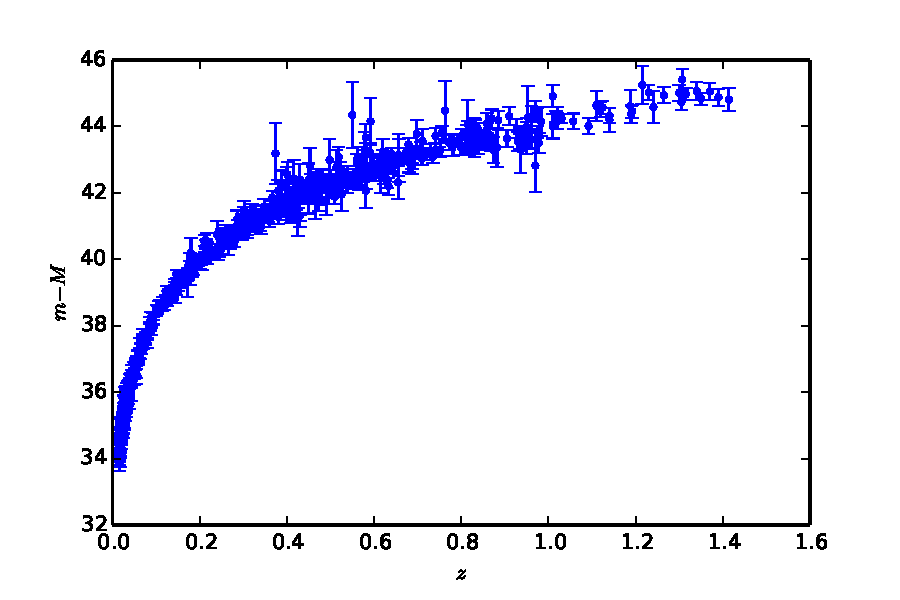
\includegraphics[width=0.48\textwidth]{fig/m-M-versus-z-con-error.pdf}
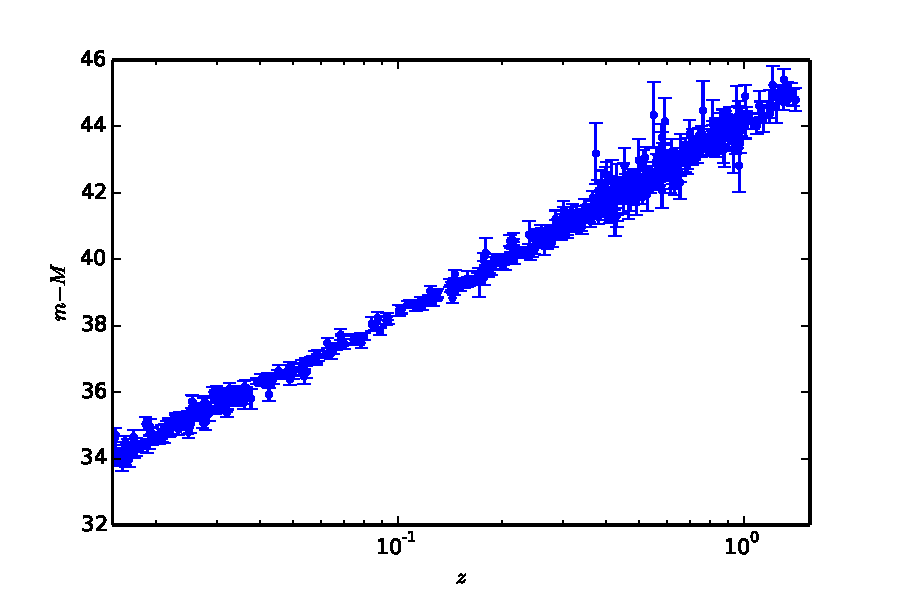
\includegraphics[width=0.48\textwidth]{fig/m-M_vs_z_semilog.pdf}
 \caption{El gr'afico superior corresponde a m-M versus redshift, mientras que el inferior es una representaci'on semilogar'itmica procedentes de supernovas tipo Ia. Ambos con barras de error.}
  \label{zvsm-M}
  \end{figure}\\
Ahora bien, de (\ref{m-M}) y (\ref{dlq0}) y usando el m'etodo de m'inimos cuadrados ponderados podemos en contrar los valores de 
$h$ y $q_0$ que se ajustan mejor a los datos (en el apendice se encuentra una secci'on con los scripts utilizados). Dichos valores
resultan ser
\begin{eqnarray}
h=0.688 \qquad; \hspace{0.5cm} q_0=-0.175\hspace{0.1cm}. 
\end{eqnarray}
Esto significa que el universo debe estar en expansi'on acelerada pues $q_0<0$. Adem'as con el valor de $h$  obtenido 
y (\ref{h}), tenemos que $H_0= 68,8 \mbox{ km s}^{-1}\mbox{Mpc}^{-1}$. Se debe mencionar tambi'en, que el valor de $q_0$
no es muy preciso, pues como se ve en los datos, hay redshifts de hasta $1.4$ lo que es bastante grande para la aproximaci'on 
a segundo orden en $z$.\\
\begin{figure}[h!]
  \centering
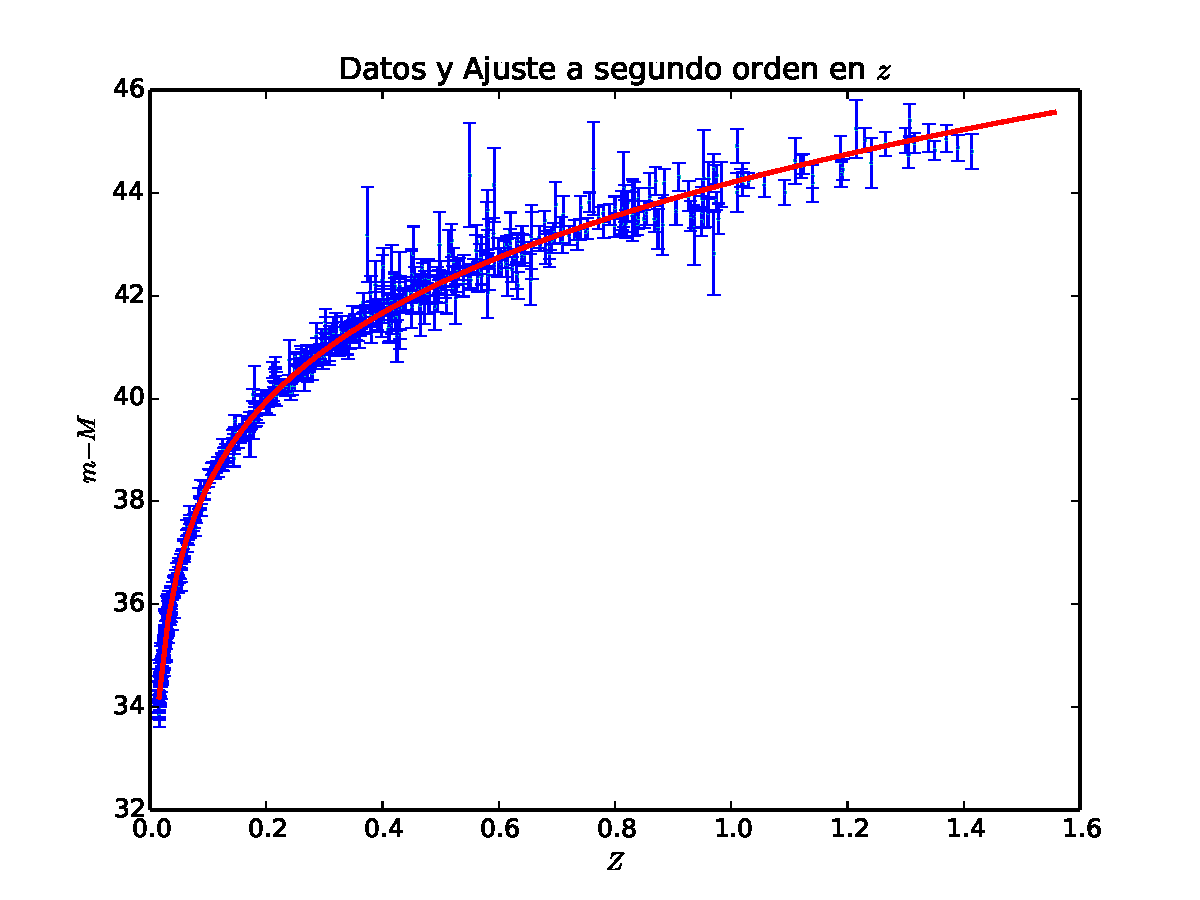
\includegraphics[width=0.7\textwidth]{fig/datos-y-ajusteq0.pdf}
 \caption{Gr'afico correspondiente al ajuste de la expresi'on a segundo orden en $z$. Con $h=0.688$ y $q_0=-0.175$.}
  \label{q000}
  \end{figure}\\
De la figura (\ref{q000}), se ve que la curva se ajusta muy bien a los datos observacionales, pero es conveniente hacer
un estudio un poco m'as profundo para dilucidar si este ajuste  es bueno. Con este propocito utilizaremos el diagrama de residuos
y su correspondiente histograma. C'omo se puede apreciar de (\ref{res}), el diagrama de residuos nuestra una distribuci'on 
m'as o menos aleatoria en torno a cero, esto significa que el ajuste pasa aproximadamente por en medio de todos los puntos. Esto
es corroborado por su histograma, ya que presenta aproximadamente una forma de distribuci'on normal\footnote{El Teorema del l'imite central establece que, bajo ciertas condiciones, la suma de un gran n'umero de variables aleatorias se aproxima a una distribuci'on normal.}. 
\begin{figure}[h!]
  \centering
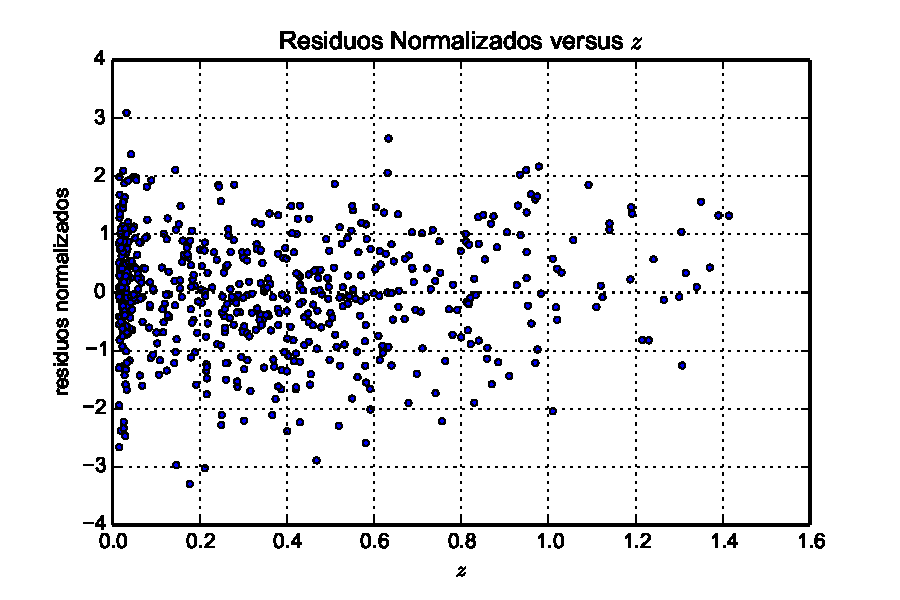
\includegraphics[width=0.48\textwidth]{fig/residuosnorq0.pdf}
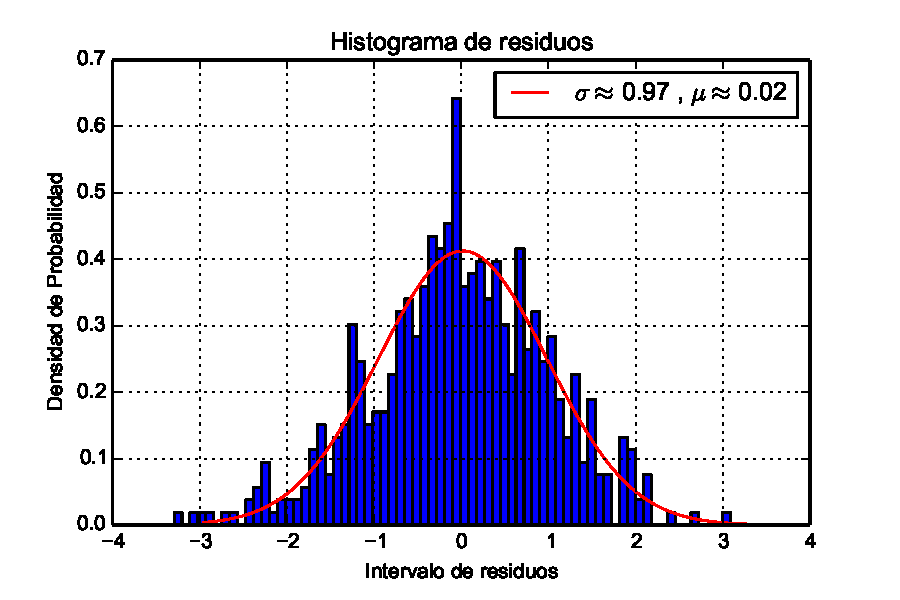
\includegraphics[width=0.48\textwidth]{fig/gaussq0.pdf}
 \caption{El gr'afico de la izquierda corresponde al diagrama de residuos del ajuste, mientras que el de la derecha corresponde 
 al histograma de residuos al cual se le ajust'o una curva gaussiana, con $\sigma^2$ la varianza y $\mu$ la media.}
  \label{res}
  \end{figure}\\ \\      
Este mismo an'alisis se puede hacer con los modelos definidos por la relaci'on (\ref{dlzk}), usando m'inimos cuadrados ponderados podemos ajustar 
los par'ametros de los 3 modelos ($k=-1,0,1$). En la figura \ref{datosyajustes} vemos los 3 modelos. Es dif'icil discernir entre cu'al de los tres
es el mejor, ya que en los 3 casos las curvas se ajustan muy bien a los datos y adem'as los valores de los par'ametros obtenidos son muy similares. Para el caso $k=-1$ se tiene
\begin{eqnarray}
h=0.7001,\quad\Omega_\Lambda=0.7237,\quad\Omega_M=0.2731,\quad\Omega_R=0.0024,\quad\Omega_k=0.0008.\hspace{0.1cm} 
\end{eqnarray}
Para el caso $k=0$,
\begin{eqnarray}
h=0.7000,\quad\Omega_\Lambda=0.7225,\quad\Omega_M=0.2773,\quad\Omega_R=0.0002,\quad\Omega_k\equiv0\hspace{1.1cm}
\end{eqnarray}
Para el caso $k=1$,
\begin{eqnarray}
h=0.7000,\quad\Omega_\Lambda=0.7231,\quad\Omega_M=0.2765,\quad\Omega_R=0.0005,\quad\Omega_k=-0.0001.
\end{eqnarray}
\begin{figure}[h!]
  \centering
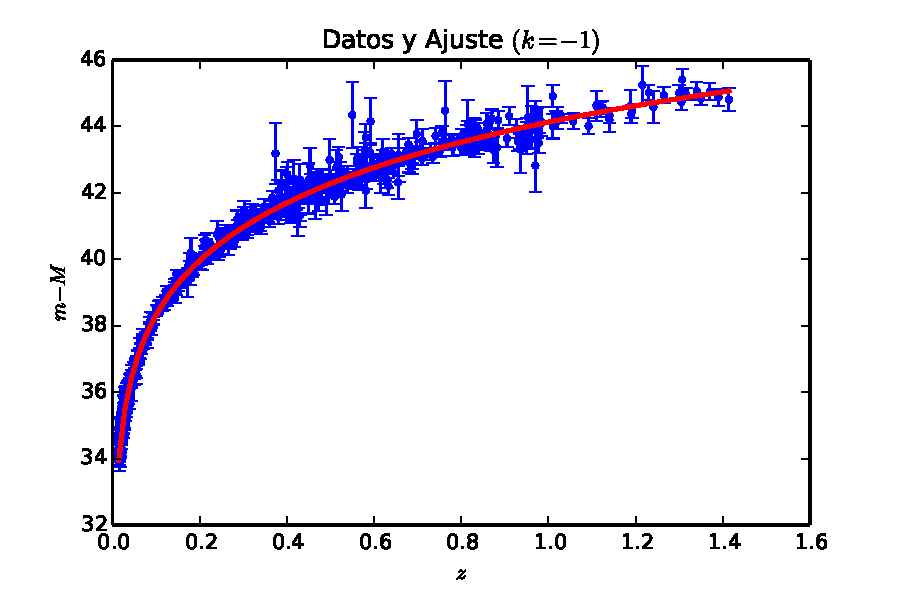
\includegraphics[width=0.49\textwidth]{fig/datos-y-ajustek-1.pdf}
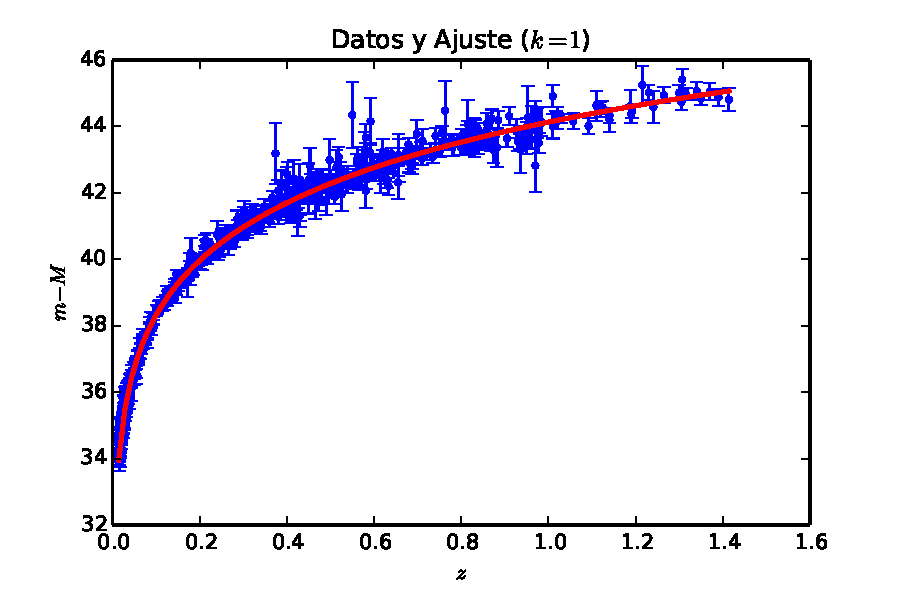
\includegraphics[width=0.49\textwidth]{fig/datos-y-ajustek1.pdf}
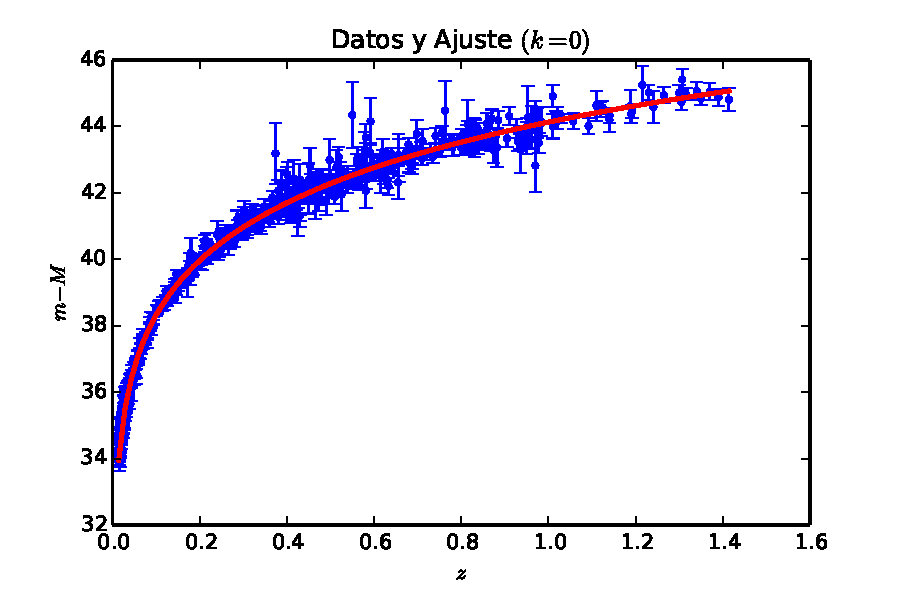
\includegraphics[width=0.60\textwidth]{fig/datos-y-ajuste.pdf}
 \caption{El gr'afico superior izquierdo corresponde al caso de un universo con curvatura espacial negativa, el superior
 derecho al caso de un universo con curvatura espacial positiva y el inferior central, al caso de un universo espacialmente plano.}
  \label{datosyajustes}
\end{figure}\\
\begin{figure}[h!]
  \centering
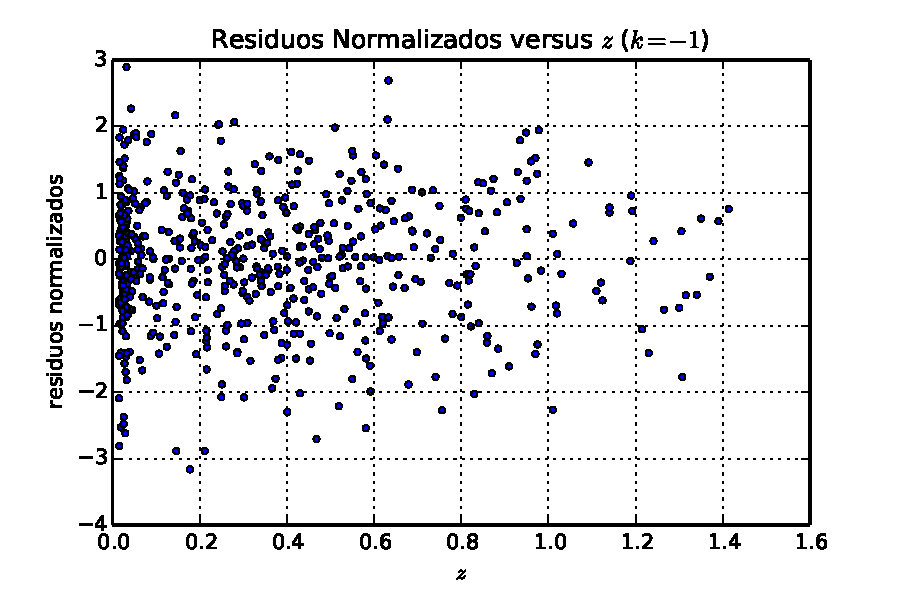
\includegraphics[width=0.49\textwidth]{fig/residuosnork-1.pdf}
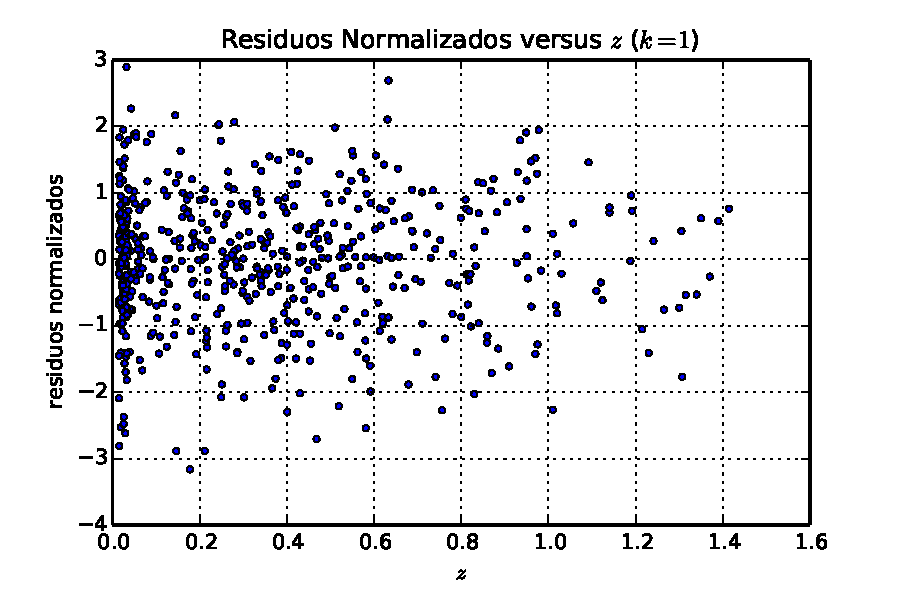
\includegraphics[width=0.49\textwidth]{fig/residuosnork1.pdf}
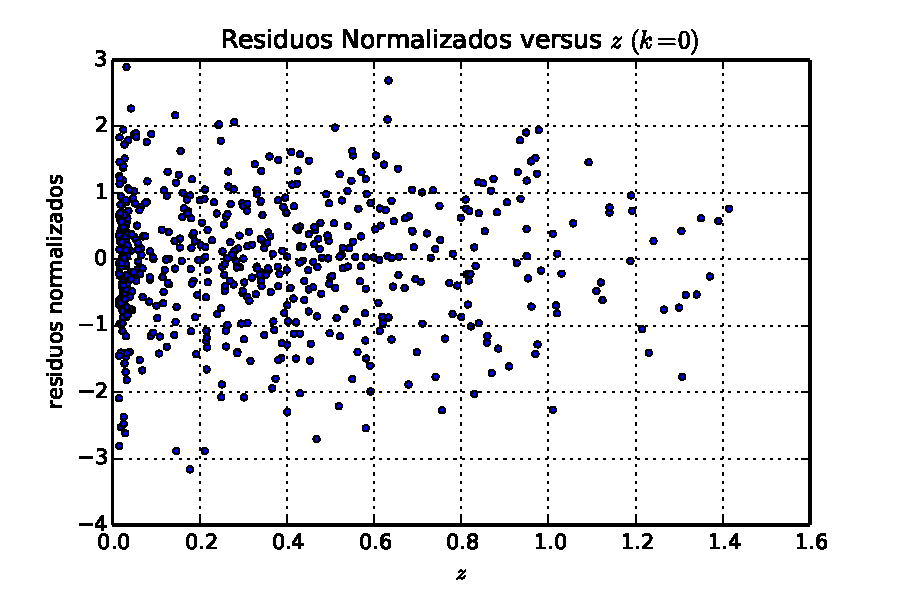
\includegraphics[width=0.55\textwidth]{fig/residuosnor.pdf}
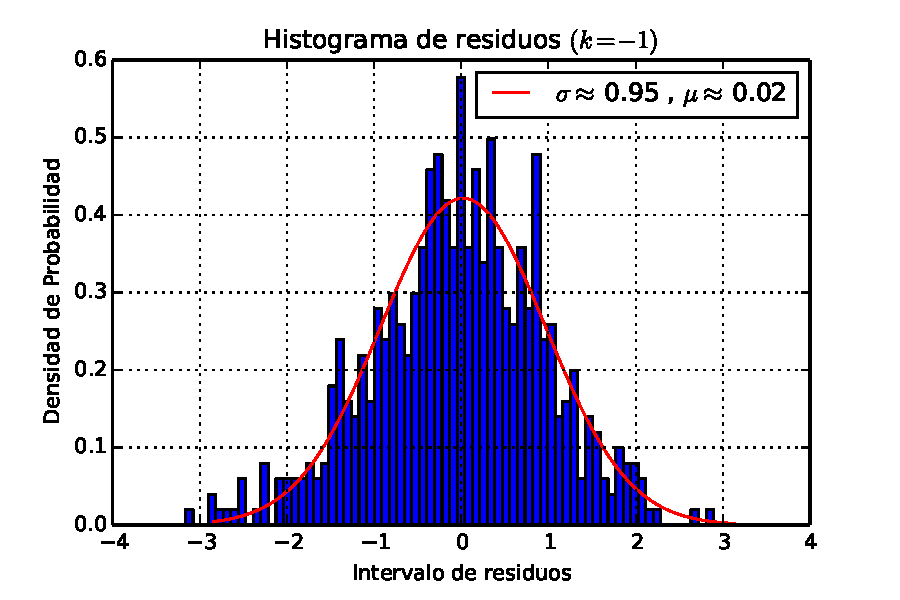
\includegraphics[width=0.49\textwidth]{fig/gaussk-1.pdf}
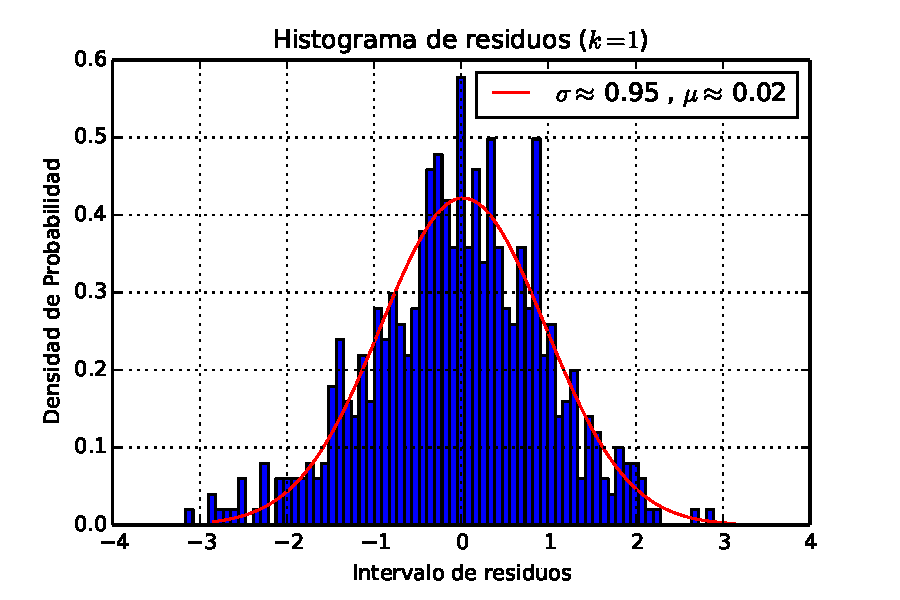
\includegraphics[width=0.49\textwidth]{fig/gaussk1.pdf}
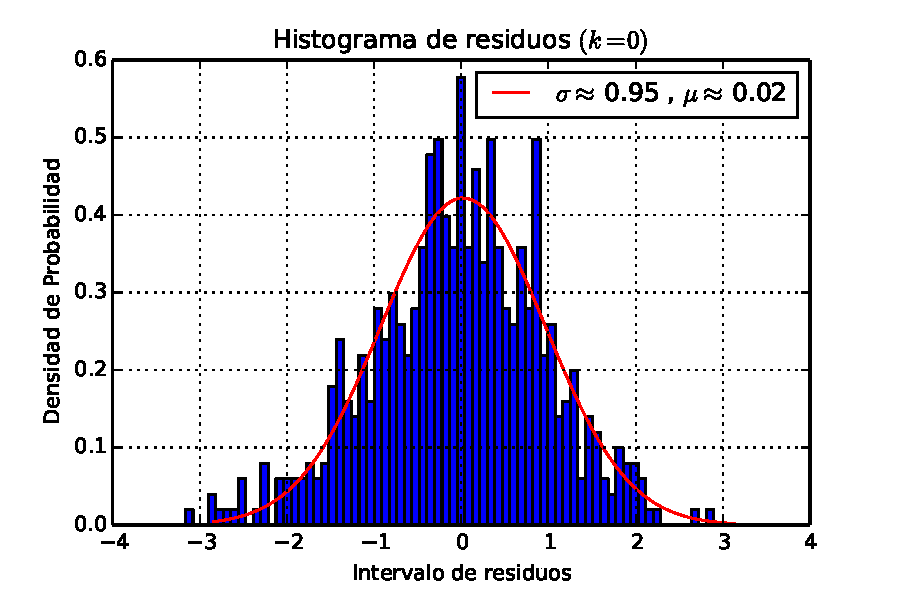
\includegraphics[width=0.55\textwidth]{fig/gaussk0.pdf}
 \caption{Diagrama de residuos correspondientes a los tres distintos valores de $k$, con sus respectivos histogramas.}
  \label{residuos}
\end{figure}\\
En los tres casos los par'ametros toman valores similares, alrededor del $73\%$ de la densidad de masa del universo es contribuida
por la constante cosmol'ogica y el $27\%$ restante es contribuido por la materia no-relativista. Por otro lado, la contribuci'on
de la materia relativista no alcanza el $1\%$. Adem'as, reemplazando en (\ref{tiempo}) los valores obtenidos, podemos
calcular las correspondientes edades del universo, que nuevamente resultan muy similares para los 3 casos.\\
\begin{equation}
\begin{array}{ll}
k=-1,& \mbox{Edad del Universo} \approx 13.66 \mbox{ miles de Millones de a\~nos}.\\
k=0, & \mbox{Edad del Universo} \approx 13.75 \mbox{ miles de Millones de a\~nos}.\\
k=1, & \mbox{Edad del Universo} \approx 13.73 \mbox{ miles de Millones de a\~nos}.\\
\end{array}
\end{equation}
As'i mismo, sus respectivos diagramas de residuos e histogramas, como vemos en la figura \ref{residuos}, presentan formas muy similares.
Por otro lado, con estos valores obtenidos y de (\ref{q0omega}) podemos obtener valores m'as precisos de $q_0$, ya que el obtenido anteriormente
proviene de una aproximaci'on a segundo orden en $z$. Para $k=-1$ se tiene que $q_0=-0.5848$, mientras que para $k=0$ se obtiene $q_0=-0.5836$, por 'ultimo,
 en el caso $k=1$ el valor obtenido es $ q_0=-0.5844$. Estos tres valores de $q_0$ son aproximadamente tres veces m'as grandes que el anteriormente
 calculado.\\
 
 Por otro lado, podemos calcular el \textit{Coeficiente de determinaci'on} de nuestros ajustes, definido como 
\begin{equation}
 R^2:=1- \frac{\sum_i(y_i-f_i)^2}{\sum_i(y_i- \bar{y})^2},
\end{equation}
con $y_i$ los datos utilizados, $f_i$ el ajuste usado y $\bar{y}$ el promedio de todos los datos. Entre m'as cercano sea $R^2$ a uno
mejor es el ajuste, por el contrario, si $R^2$ se aproxima a cero entonces el ajuste no es muy confiable.\\
Los coeficientes de determinaci'on obtenidos fueron:
\begin{equation}
\begin{array}{rl}
\mbox{Aproximaci'on a segundo orden en $z$:}& R^2 = 0.992795,\\
\mbox{Modelo con $k=-1$:}& R^2 = 0.993036,\\
\mbox{Modelo con $k=0$:} & R^2 = 0.993036, \\
\mbox{Modelo con $k=1$:} & R^2 = 0.993036.
\end{array}
\end{equation}
Como es de esperarse, la aproximaci'on a segundo orden en $z$, no es tan buena como los ajustes de los tres modelos, pues es s'olo una 
aproximaci'on. Por otro lado, el coeficiente de determinaci'on no nos permite distinguir qu'e modelo del universo es mejor ($k=-1,0,1$).\\
 
 
Pero a'un no hemos corroborado la importancia de la constante cosmol'ogica. Ya que todos los modelos son muy parecidos, consideraremos $k=0$ por su simplicidad. 
En la figura \ref{parametros}, hemos graficado nuestro modelo con valores de $\Omega_\Lambda$, $\Omega_R$ y $\Omega_M$ asignados por nosotros. Para las tres curvas
elegimos $h=0.7$.
\begin{figure}[h!]
  \centering
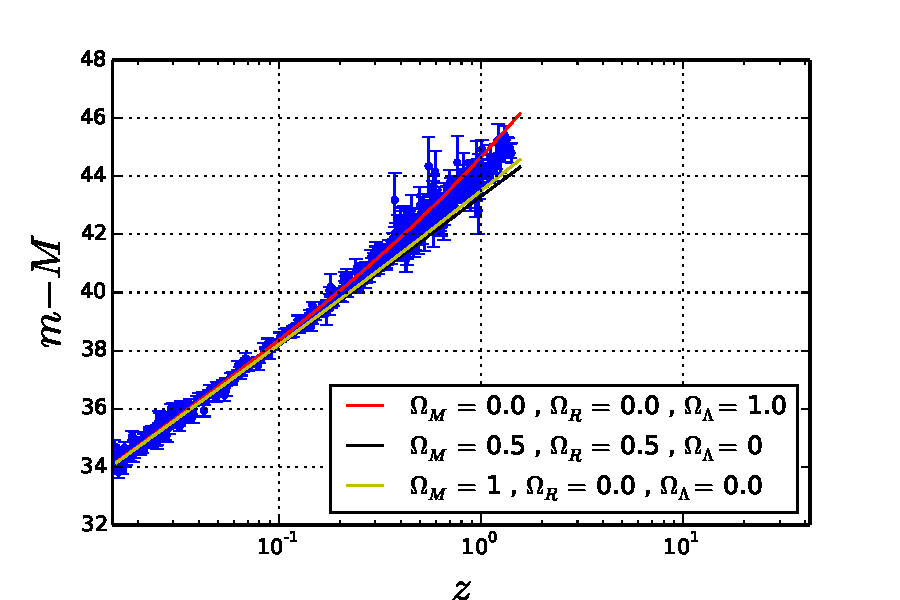
\includegraphics[width=0.49\textwidth]{fig/parametros_de_prueba.pdf}
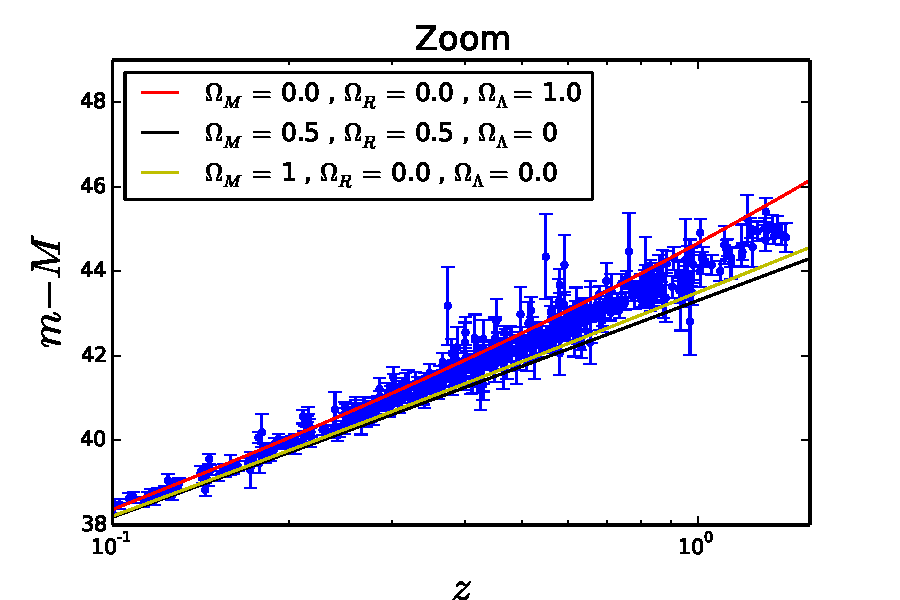
\includegraphics[width=0.49\textwidth]{fig/zoom.pdf}
 \caption{El gr'afico de la izquierda corresponde a las curvas del modelo con $k=0$, para algunos valores de los par'ametros asignados por nosotros. 
 El gr'afico de la derecha corresponde a un zoom de la parte superior del gr'afico de la izquierda. Las tres curvas para redshifts peque\~nos se ajustan bien los datos, pero para redshifts mayores toma mayor importancia el
 tipo de materia presente en el universo.}
  \label{parametros}
\end{figure}\\
En el caso l'imite de un universo vac'io, s'olo con constante cosm'olgica (la curva de color rojo), el modelo predice una expansi'on mayor a la observada. Por otro lado, en un universo
s'olo con materia relativista y no-relativista (curva de color negro), predice una expansi'on menor a la observada. En sus respectivos diagramas de residuos se
ve que hay tendencias que se dejan fuera para estos dos casos.\\
%Recordemos que introdujimos las constante cosmol'ogica para poder describir la expansi'on acelerada del universo, en su aucencia
\begin{figure}[h!]
  \centering
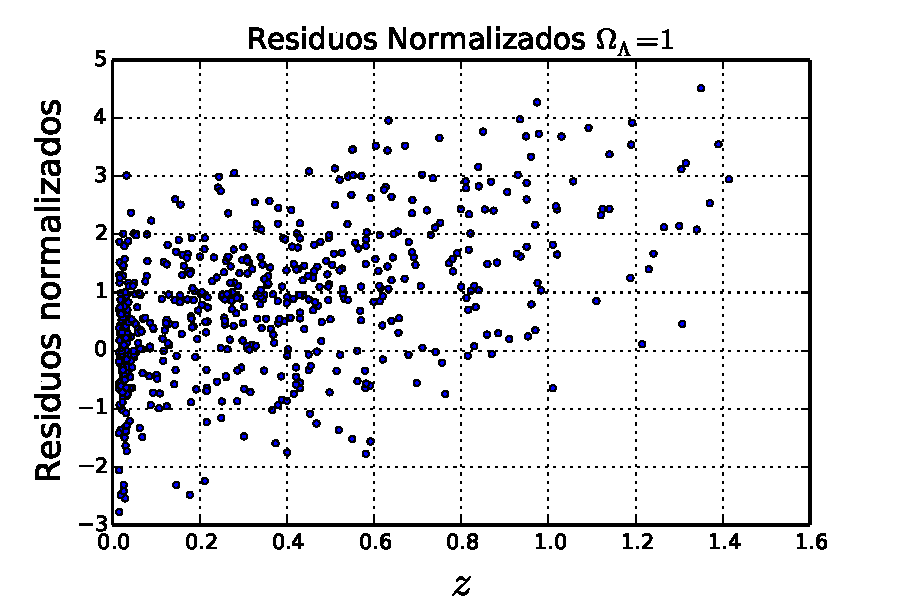
\includegraphics[width=0.49\textwidth]{fig/resparametros1.pdf}
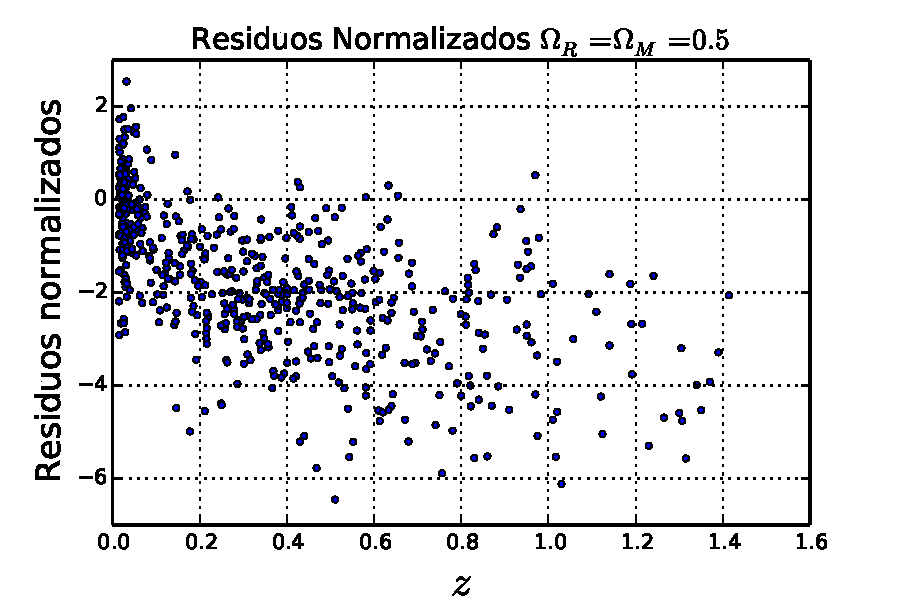
\includegraphics[width=0.49\textwidth]{fig/resparametros3.pdf}
 %\caption{}
  \label{parametros2}
\end{figure}\\
Adem'as, podemos elegir de antemano $\Omega_\Lambda=0$ y usar el m'etodo de m'inimos cuadrados para ajustar (\ref{dlzk}) a los datos.  
\begin{figure}[h!]
  \centering
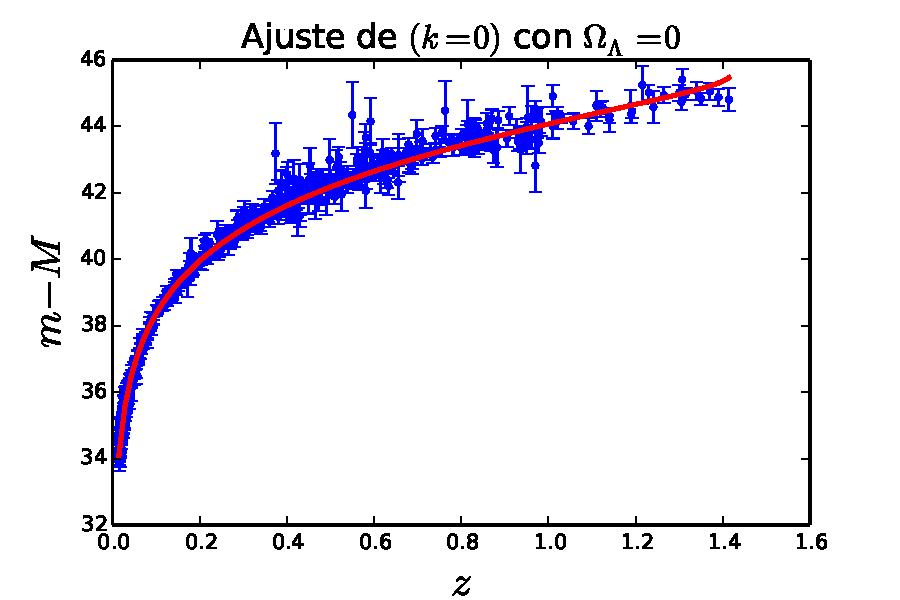
\includegraphics[width=0.70\textwidth]{fig/datos-y-ajustelambda0.pdf}
 %\caption{}
  \label{lambda0}
\end{figure}\\     
La curva se ajusta muy bien a los datos, y parece no ser necesaria la constante cosmol'ogica, pero el valor obtenido de los par'ametros ajustados son:
$h= 0.6645$, $\Omega_M=1.7057$ y $\Omega_R=-0.7057$. Es claro que esto se aleja de la realidad f'isica del problema, pues $\rho_R>0$.
Por lo que, la constante cosmol'ogica es necesaria en este modelo del universo.

Por otro lado, podemos hacer un an'alisis estad'istico de nuestros ajustes, con los contornos de confianza (confidence contours) de los
par'ametros ajustados. Esto es un intervalo de n'umeros entre los cuales se estima que estar'a cierto valor
desconocido con una determinada probabilidad de acierto. Esta probabilidad se calcula a partir de datos de una muestra, y los valores desconocidos
son los par'ametros a ajustar. La probabilidad de 'exito en la estimaci'on se representa con $1-\alpha$ y se denomina nivel de confianza. Aqu'i $\alpha$ 
es el llamado error aleatorio o nivel de significaci'on y es una medida de las posibilidades de fallar en la estimaci'on mediante tal intervalo.
El nivel de confianza y la amplitud del intervalo var'ian conjuntamente, de forma que un intervalo m'as amplio tendr'a m'as probabilidad
de acierto (mayor nivel de confianza). Mientras que, para un intervalo m'as peque\~no, la estimaci'on es m'as precisa, pero aumenta su
probabilidad de error. Es habitual que el par'ametro presente una distribuci'on normal.

Los valores m'inimos de $\chi^2$ en los cuatro casos son:


\begin{eqnarray}
\mbox{Aprox. a segundo orden en $z$}: \qquad \chi^2\approx581.39,\\
\mbox{Expresi'on completa, caso $k=-1$}: \qquad \chi^2\approx 562.23,\\
\mbox{Expresi'on completa, caso $k=0$}:  \qquad \chi^2\approx 562.23,\\
\mbox{Expresi'on completa, caso $k=1$}:  \qquad \chi^2\approx 562.23.
\end{eqnarray}
\begin{figure}[h]
  \centering
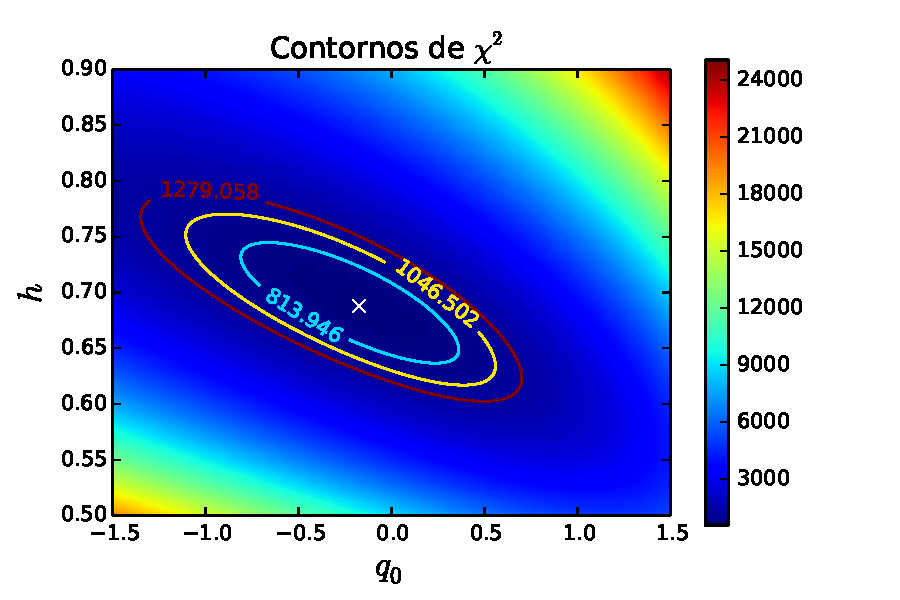
\includegraphics[width=0.65\textwidth]{fig/contornoq0.pdf}
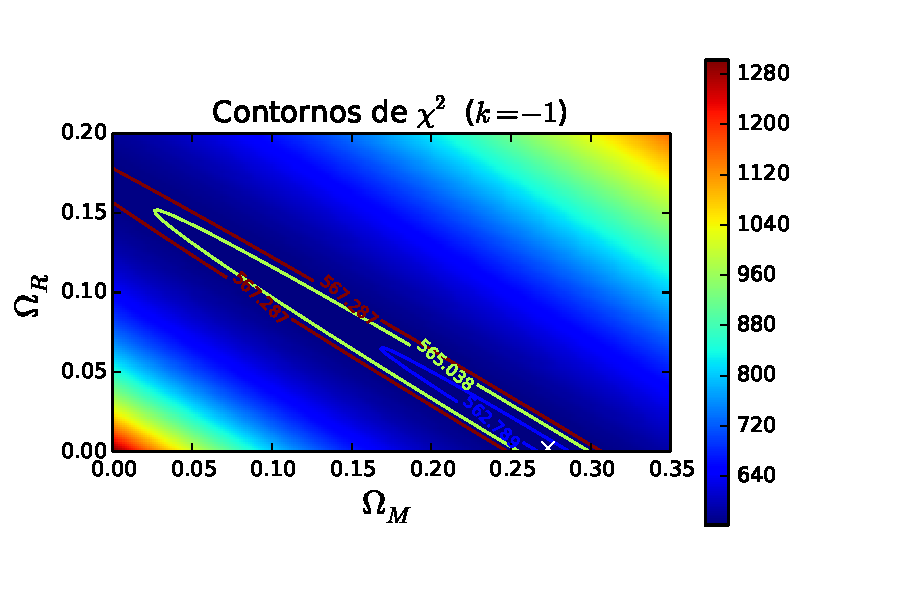
\includegraphics[width=0.65\textwidth]{fig/contornok-1.pdf}
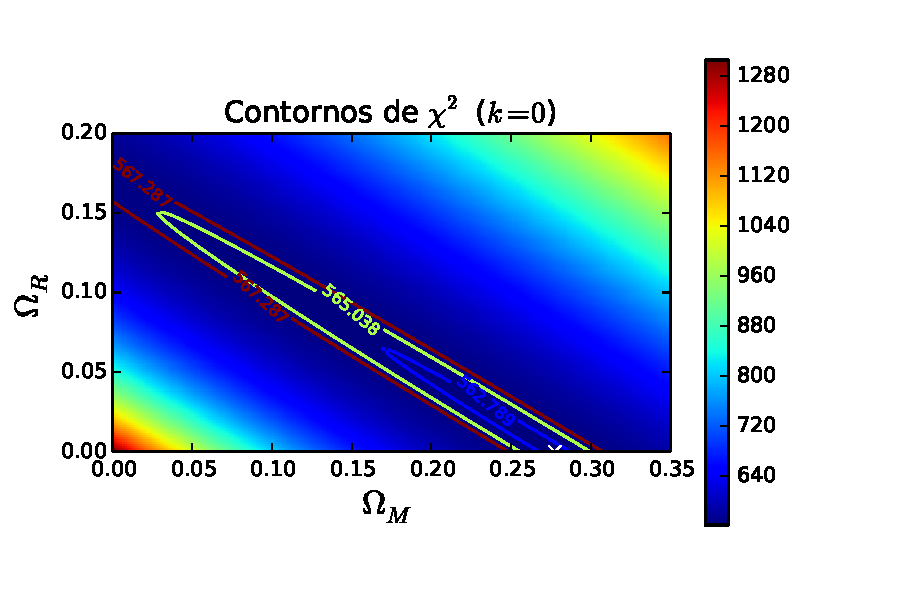
\includegraphics[width=0.65\textwidth]{fig/contornok0.pdf}
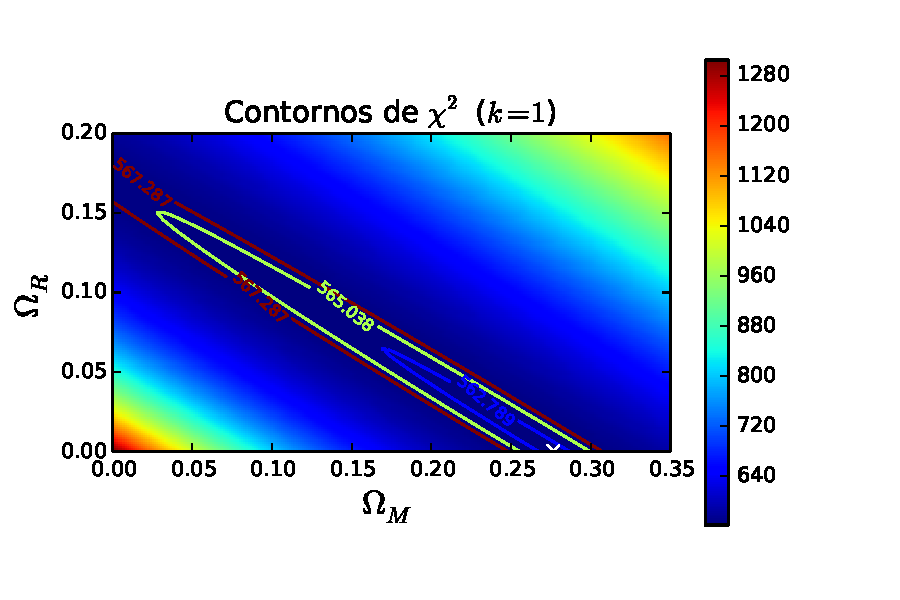
\includegraphics[width=0.65\textwidth]{fig/contornok1.pdf}
 \caption{Contornos de confianza de nuestros modelos. La barra lateral indica el valor de $\chi^2$ dependiendo del valor de los par'ametros. Los
 valores de $h$ y $\Omega_k$ utilizados son los obtenidos por m'inimos cuadrados en cada caso. La x el punto en que $\chi^2$ alcanza su valor m'inimo.}
  \label{parametros22}
\end{figure}

Por otro lado, como la estad'istica de $\chi^2$ es una variable aleatoria, se le puede asignar una distribuci'on de probabilidad, dada por
\begin{eqnarray}
X(\chi^2;\nu)= \frac{(\chi^2)^{(\frac{\nu}{2}-1)}\exp[-\chi^2/2]}{2^{\nu/2}\Gamma(\nu/2)}, \qquad \mbox{con} \qquad \nu=\mbox{N}-\mbox{\textit{N}}.
\end{eqnarray}
Donde $\nu$ son los grados de libertad del ajuste, es decir, es el n'umero de datos usados menos el n'umero de par'ametros a ajustar. En la
figura \ref{parametros3} se muestra el gr'afico correspondientes a la densidad de probabilidad de $\chi^2$.\\ 
\begin{figure}[h!]
  \centering
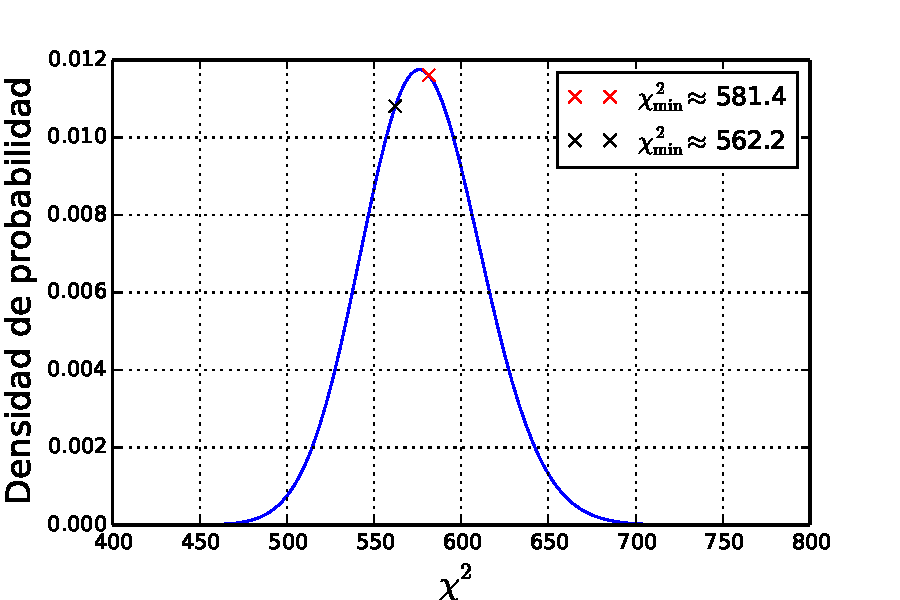
\includegraphics[width=0.60\textwidth]{fig/densidadq0.pdf}
%\includegraphics[width=0.49\textwidth]{densidadk-1.pdf}
%\includegraphics[width=0.49\textwidth]{densidadk0.pdf}
%\includegraphics[width=0.49\textwidth]{densidadk1.pdf}
 \caption{Densidad de probablidad de $\chi^2$. 'Esta se calcul'o usando 580 datos y usando dos par'ametros libres para ajustar. En el caso de la proximaci'on en 
 $z$ los parametros son $h$ y $q_0$. Por otro lado, para la expresi'on completa, se fijaron $h$ y $\Omega_k$ en los valores que minimizan $\chi^2$, $\Omega_M$ y $\Omega_R$ fueron los considerados como par'ametros a ajustar.
 La x roja corresponde al valor de $\chi^2_{\rm{min}}$ con la aproximaci'on a segundo orden en $z$ y la x negra corresponde al valor $\chi^2_{\rm{min}}$ usando la expresi'on completa. El valor 'optimo de $\chi^2$ seg'un su 
 distribuci'on de probabilidad es de aproximandamente 576.9.} 
  \label{parametros3}
\end{figure}\\         
Con esta expresi'on podemos calcular la probabilidad de encontrar alg'un $\chi^2$ entre el valor m'inimo de $\chi^2$ ($\chi^2_{\rm{min}}$) e $\infty$ , como:
\begin{equation}
P(\chi^2_{min}\leq\chi^2\leq\infty;\nu)=\int^{\infty}_{\chi^2_{\rm{min}}}X(\chi^2;\nu)d\chi^2.
\end{equation}
Pero, por otro lado esta probabilidad est'a normalizada, entonces
\begin{equation}
 1=\int^{\infty}_0 X(\chi^2;\nu)d\chi^2,
\end{equation}
luego, podemos escribir 
\begin{equation}
P(\chi'^2\leq\chi^2\leq\infty;\nu)=1- \int^{\chi'^2}_0 X(\chi^2;\nu)d\chi^2 = 1 -\alpha.
\end{equation}
'Este es el porcentaje de probabilidad de obtener un valor de $\chi^2 \geq \chi'^2$. \\ \\ \\

Entonces, hemos visto que el universo se est\'a expandiendo y lo hace en forma acelerada. Adem\'as, en este modelo del universo es 
necesaria la constante cosmolo\'ogica en las ecuaciones de Einstein para podemer explicar la expansi\'on acelerada. En los tres modelos
del universo, alrededor del $73\%$ de la densidad de masa del universo es contribuida por la constante cosmol'ogica y el $27\%$
restante es contribuido por la materia no-relativista. Con los diagramas de residuos e histogramas pudimos verificar que tan buenos fueron
los ajustes, en particular, s\'olo con los datos de las supernovas no es posible dilucidar cual es el caso que se ajusta mejor a los datos.